\chapter{Gas Electron Multiplier} % (fold)
\label{cha:gas_electron_multiplier}
\begin{chapquote}
{Freeman Dyson}
``New directions in science are launched by new tools much more often than by new concepts.''
\end{chapquote}

In this chapter, the GEM detector technology is introduced which are proposed for the CMS muons system upgrade during the long shutdown-2 period. 
The properties of these GEM detectors were scrutinized during different beam test campaigns carried out at the CERN SPS beam test facility.
The first half of this chapter deals with the measurements performed on prototypes of CMS GEM detectors using the data collected during  different beam tests. 
The characterisation of GEM foils developed in India for the CMS upgrade is described in the last part of the chapter.

\section{Introduction} % (fold)
\label{sec:introduction}
The invention of Multi-Wire Proportional Chamber (MWPC) in 1968 by Georges Charpak was one of the major breakthroughs in the development of gaseous detectors since it had better rate capability vis-a-vis its predecessors~\cite{Charpak1968}. 
This invention also leads to a Nobel prize for George Charpak in 1992. 
The design and performance of MWPC have improved progressively through all these years.
However, because of our increasing demands with the acquired knowledge about particle detection, it has reached its limitation in terms of the maximum rate capability and detector granularity.
In 1988, Anton Oed invented the Micro-Strip Gas Counter (MSGC) which had a position resolution of few tens of microns and could overcome the rate limitation arising due to positive-ion accumulation in the gas volume. 
Also, it could sustain a particle flux greater than few $MHz/mm^2$. Although, these kind of detectors were very impressive but the long-term study revealed the following shortcomings:
\begin{enumerate}
	\item Accumulation of the ions on the electrodes, which affects the gain and age of the detector.
	\item In some cases, the passage of highly ionising particles could lead to a destructive discharge in the detector medium.
\end{enumerate}
These drawbacks of the MSGC lead to the development of Micro-Pattern Gaseous Detector (MPGD).
This class of detector, specifically the Gas Electron Multiplier (GEM)~\cite{Sauli1997,Sauli1999,detector:1732870}, could provide an unprecedented spatial resolution, larger sensitive/detection area, with higher rate capability and good operational stability over the longer operating periods.
Several new studies also revealed that under certain circumstances these detectors might be less vulnerable to the radiation-induced ageing than the standard silicon microstrip detectors~\cite{TITOV2004,Titov2002}.

Because of their efficient detection qualities and high rate capabilities, GEM detectors have been already used in various experiments like COMPASS, TOTEM, LHCb. Recently, it is proposed for the CMS muon detector system upgrade. A brief description of the working and properties of GEM detectors is provided in the following sections.
% section introduction (end)

\section{Design and working principle of GEM detector} % (fold)
\label{sec:design_and_working_principle_of_gem}

GEM is a relatively new concept introduced by Fabio Sauli at CERN~\cite{Sauli1997}, which consists of a thin polyimide sheet (usually a thin Kapton foil~\cite{Kapton-sheet} with thickness 50 $\mu m$) coated with metal on its both sides. It is chemically pierced to a regular array of holes using the photolithography and acid etching processes~\cite{Benlloch1998}, as shown in Fig.~\ref{fig:gem} (left).
\begin{figure}[!htbp]
    \centering
    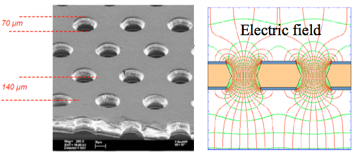
\includegraphics[width=0.95\textwidth]{figures/GEM/KEKDTP3.jpg}
    \caption{A cross-sectional view of a GEM foil etched with holes (left). The strong electric field generated in the vicinity and inside of the holes on the application of the potential across the foil (right).}
    \label{fig:gem}
\end{figure}

A potential difference is applied between the two copper layers which create a high electric field inside the holes (Fig.~\ref{fig:gem}) and is given as
\begin{equation}
    E = \frac{V}{d}
\end{equation}
where E is the electric field inside a hole in the GEM foil, V is the voltage applied between the two copper layers and d is the thickness of the GEM foil.
% Since the Kapton\footnote{Kapton was chosen as the insulating layer as it has very good insulating power along with that it can sustain very high radiation along with that it works with wide range of temperature. It is a plastic polyamide created by DuPont.} foil is very thin, around 50 $\mu m$, so a high electric field density will be created in the hole which is shown in Fig.~\ref{fig:gem} (right).
\begin{figure}[htbp]
    \centering
    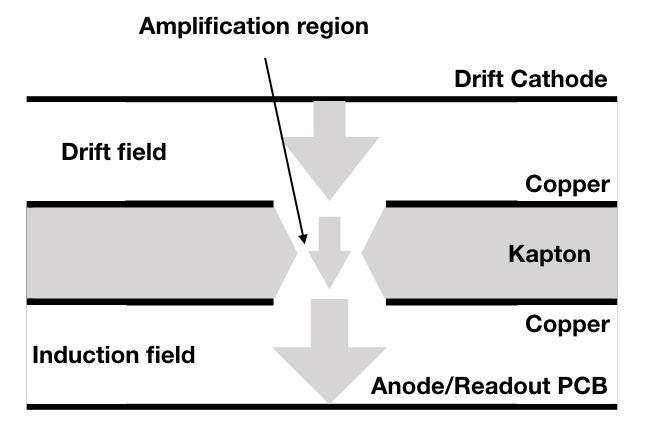
\includegraphics[width=0.55\textwidth]{figures/GEM/SingleGEM_Detector.jpeg}
    \caption{Outline of a single GEM detector.}
    \label{fig:gemOutline}
\end{figure}

To illustrate the working of a GEM detector, the active detector medium could be divided into three different regions: drift, amplification and induction regions, as shown in Fig.~\ref{fig:gemOutline}.
The passage of a charged particle leads to ionization in the drift region, and the generated primary electrons drift towards the amplification region (i.e., GEM holes). 
The electrons gain kinetic energy from the intense electric field inside the holes sufficient to produce secondary ionizations, eventually, leading to an avalanche multiplication, as shown in Fig.~\ref{fig:gem}(right).
Finally, in the induction region, all the electrons from the amplification region are collected on the readout plane. 

To avoid the problem of electrical breakdown, several GEM foils operating at lower voltages, are stacked together in between the drift cathode and the readout board.
For such detector configurations, the through transfer region takes most of the almost all the electrons from one GEM foil to another.
In view of the fact that the total gain of a detector is given as the product of the individual gain of each foil, gains up to an order of $10^5$ can be achieved in this way.
In this configuration, the detector can reach its maximum gain without any or with the least probability of electric discharge.

% Also, the total gain is the product of the individual gain of each foil, so the gain up to $10^5$ can be achieved in this way.
% In this configuration, it can reach maximum gain without any discharge or least probable.
% In Fig.~\ref{fig:tripleGEM_discharge_gain}, 
The gain and discharge probability are compared for the single, double and triple-layered GEM detectors are shown in Fig.~\ref{fig:tripleGEM_discharge_gain}, which clearly indicates that the triple GEM detectors can achieve a gain beyond $10^4$ without any electrical discharge.
Also, the signal readout by the electrode is pretty fast as it uses only electrons to read the signal. 
Multi-layered boards could be used to achieve a two-dimensional readout from these detectors.
\begin{figure}[!htbp]
    \centering
    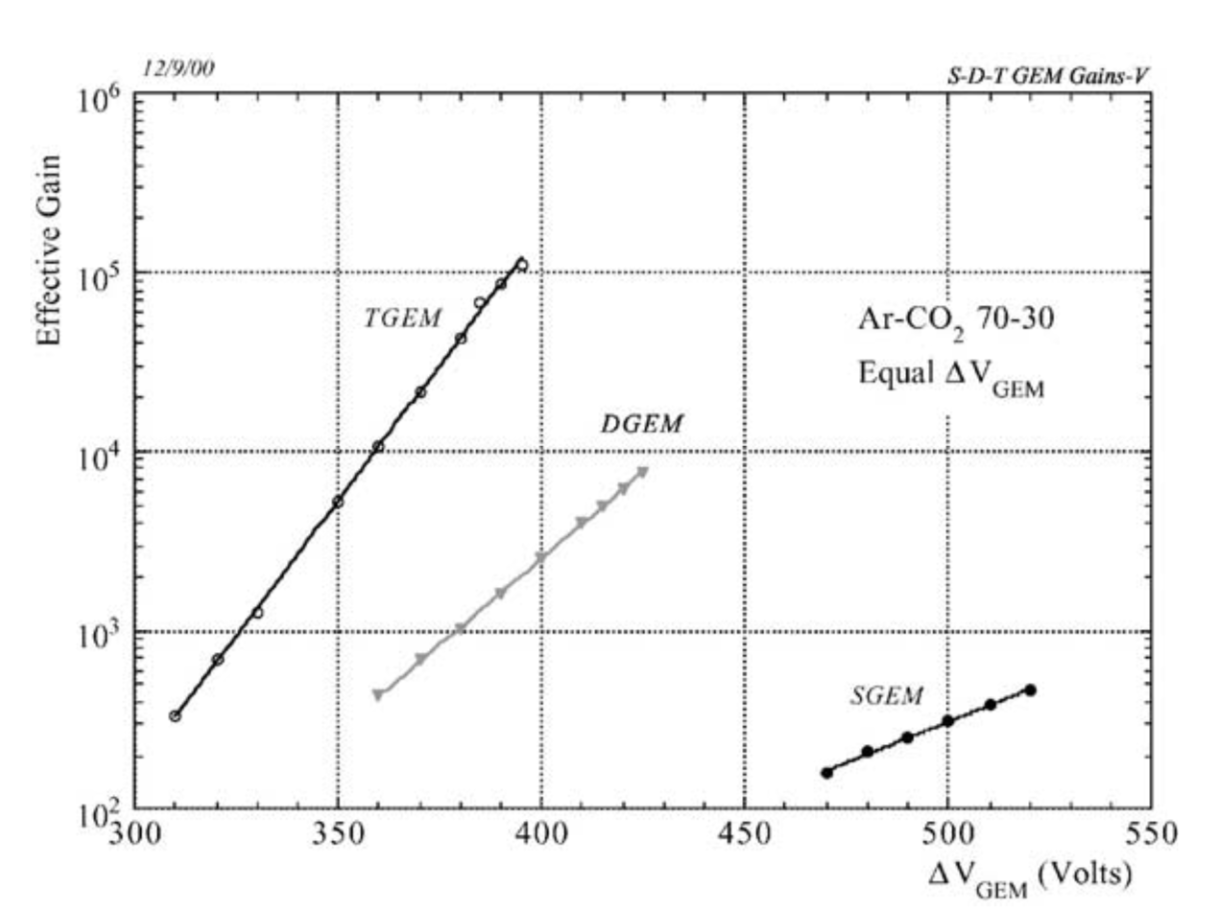
\includegraphics[width=0.5\textwidth]{figures/GEM/Comp_threeGEMS_Gain.png}%
    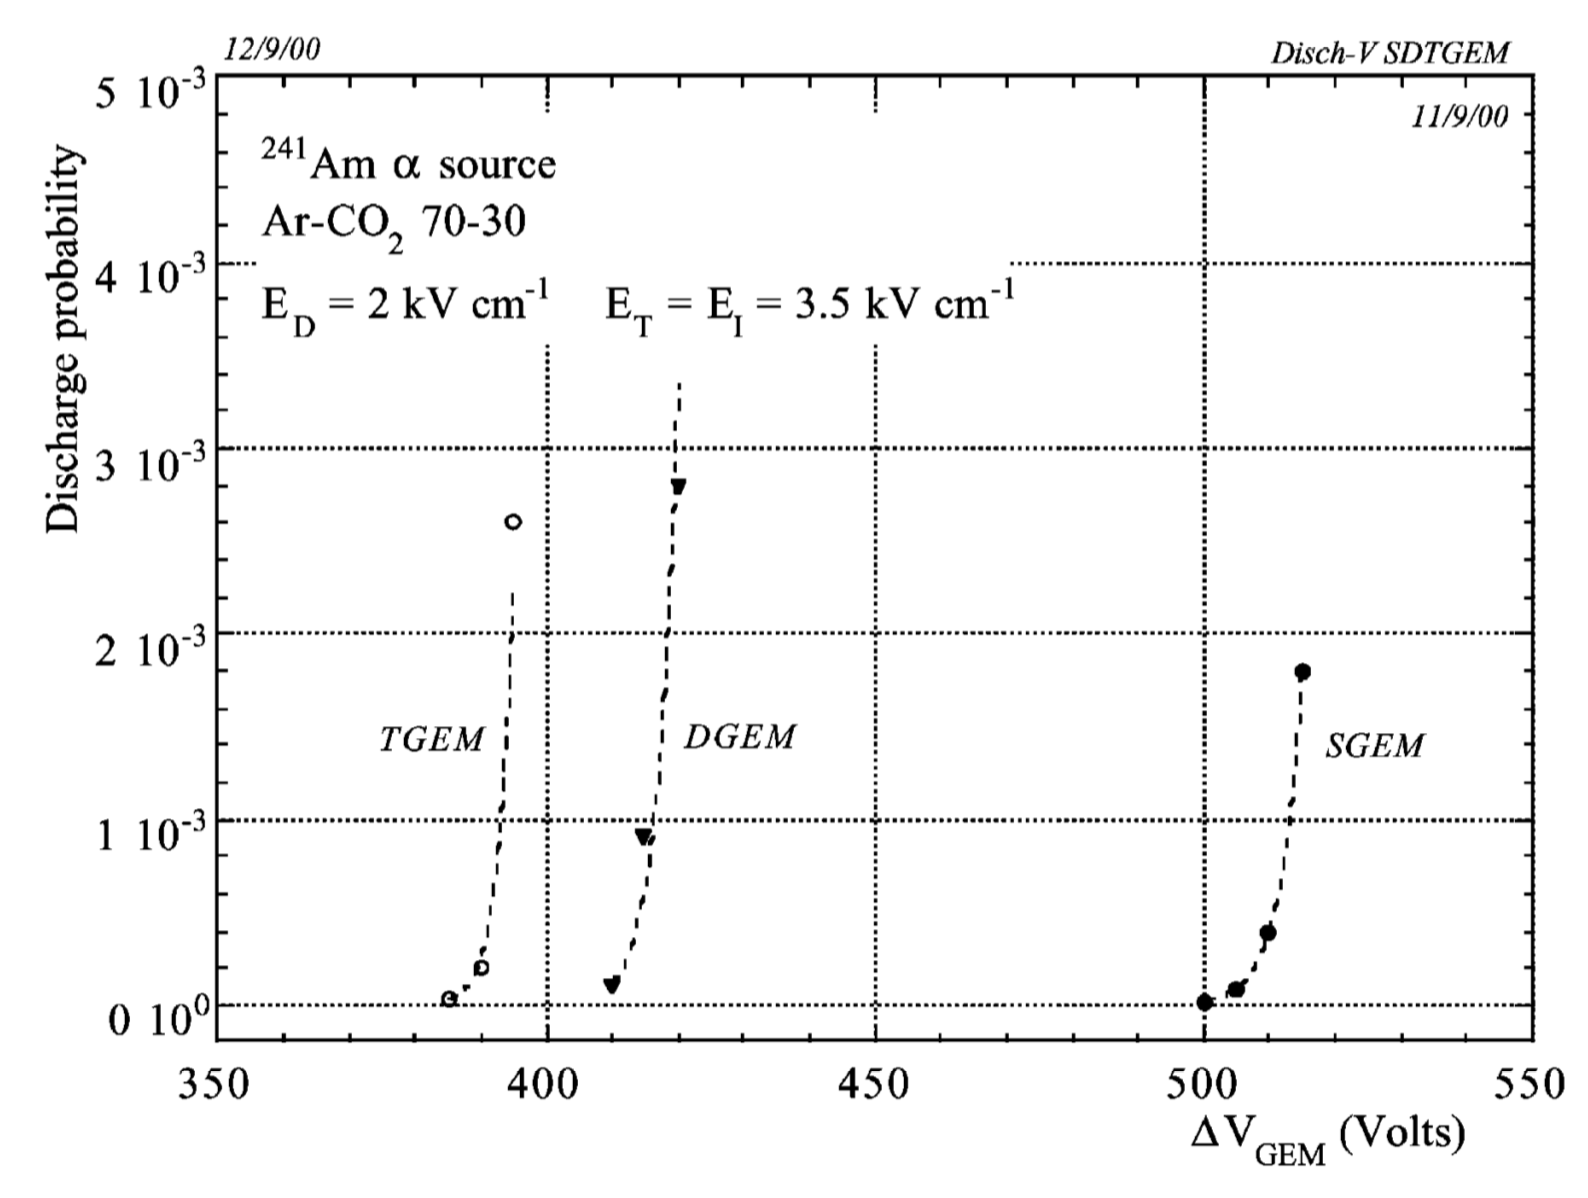
\includegraphics[width=0.5\textwidth]{figures/GEM/Comp_threeGEMS_DischargeProbability.png}
    \caption{Comparison of total effective gain on anode as a function of applied voltage for single, double and triple layred GEM detectors (left). The discharge probality as a function of applied voltage is shown for the single, double and triple layred GEM detectors (right)~\cite{Bachmann2002}.}
    \label{fig:tripleGEM_discharge_gain}
\end{figure}

A detector arrangement where three GEM foils are stacked together is known as a ``\textit{ \textbf{Triple-GEM detector}}'', as shown in Fig.~\ref{fig:gemgaps}. Such a detector configuration is proposed for the CMS Phase-II upgrade and is discussed in the following section.
\begin{figure}[!htbp]
    \begin{center}
        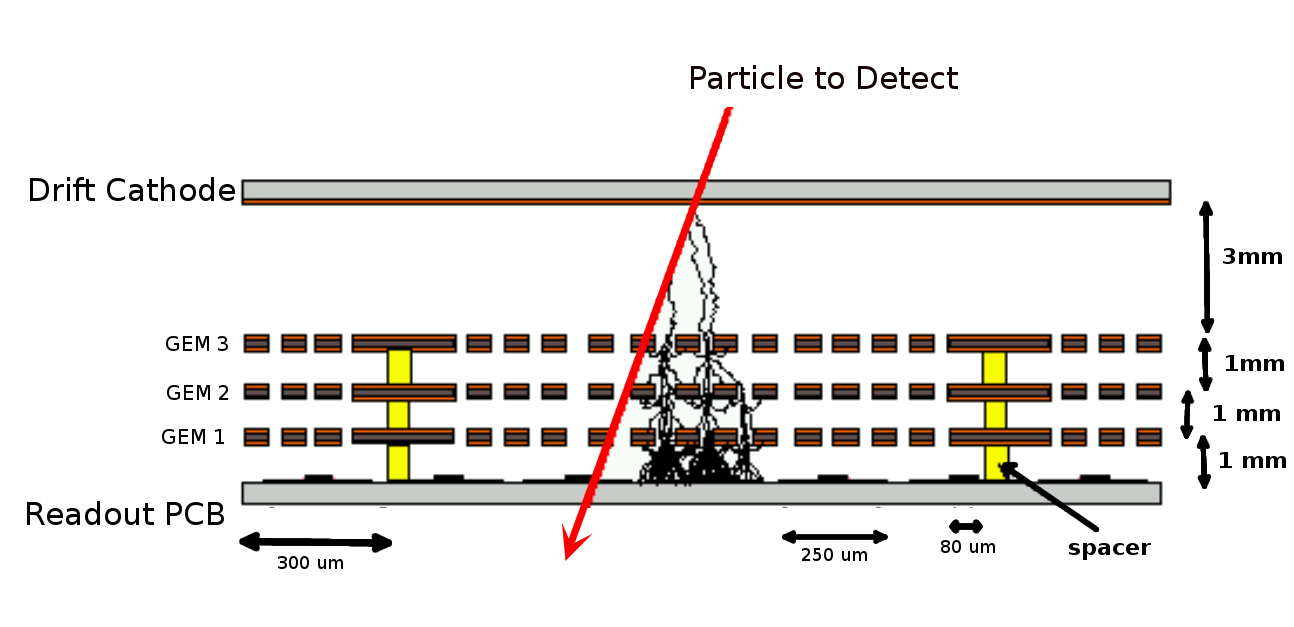
\includegraphics[width=0.85\textwidth]{figures/GEM/triple_gem.png}
        \caption{The working mechanism of a GEM detector.}
        \label{fig:gemgaps}
    \end{center}
\end{figure} 
% section design_and_working_principle_of_gem (end)


\section{GEM for the CMS Phase-II Upgrade} % (fold)
\label{sec:gem_for_cms}
As pointed out in Sec.~\ref{sub:the_muon_system},  the CMS Collaboration has finalised to install GEM detectors in the pseudo-rapidity region $1.6 < |\eta| < 2.2$.
These detectors will support the existing CSC muon sub-system to improve the muon triggering and tracking capabilities in the forward region~\cite{Colaleo:2021453}.
The combined operation of CSC and GEM detectors will lead to a precise measurement of the muon bending angle at the trigger level, thus strongly reducing the rate of muon mis-reconstruction.

This CMS muon detector system upgrade is carried out to achieve the following goals:
\begin{itemize}
    \item Re-establish the redundancy in the forward region beyond $\eta = 1.6$
    \item Improve the muon tracking performance during the high-luminosity LHC operation.
    % \item The combined operation of CSC and GEM detectors allows a measurement of the bending angle at the trigger level, thus strongly reducing the rate of mis-measured muons driving the triggers rate.
\end{itemize}
% \subsection{GE1/1 Details}
The installation of GEM detectors is proposed during the period of Long Shut down-2 (2019-2020).
The upgrade project is named as CMS GE1/1 upgrade, where the letter ``G'' stands for GEM, ``E'' stands for End-cap, the first ``1'' corresponds to the first muon station and the second ``1'' corresponds to the first ring of the station.
Analogously, the GEM detectors to be installed in the CMS detector are referred to as GE1/1 detectors.
The detectors will be inserted in front of the ME1/1 station and into the slots originally foreseen for the RPC detectors, as shown in Fig.~\ref{fig:GE1/1pos}. 
\begin{figure}[!htbp]
    \centering
    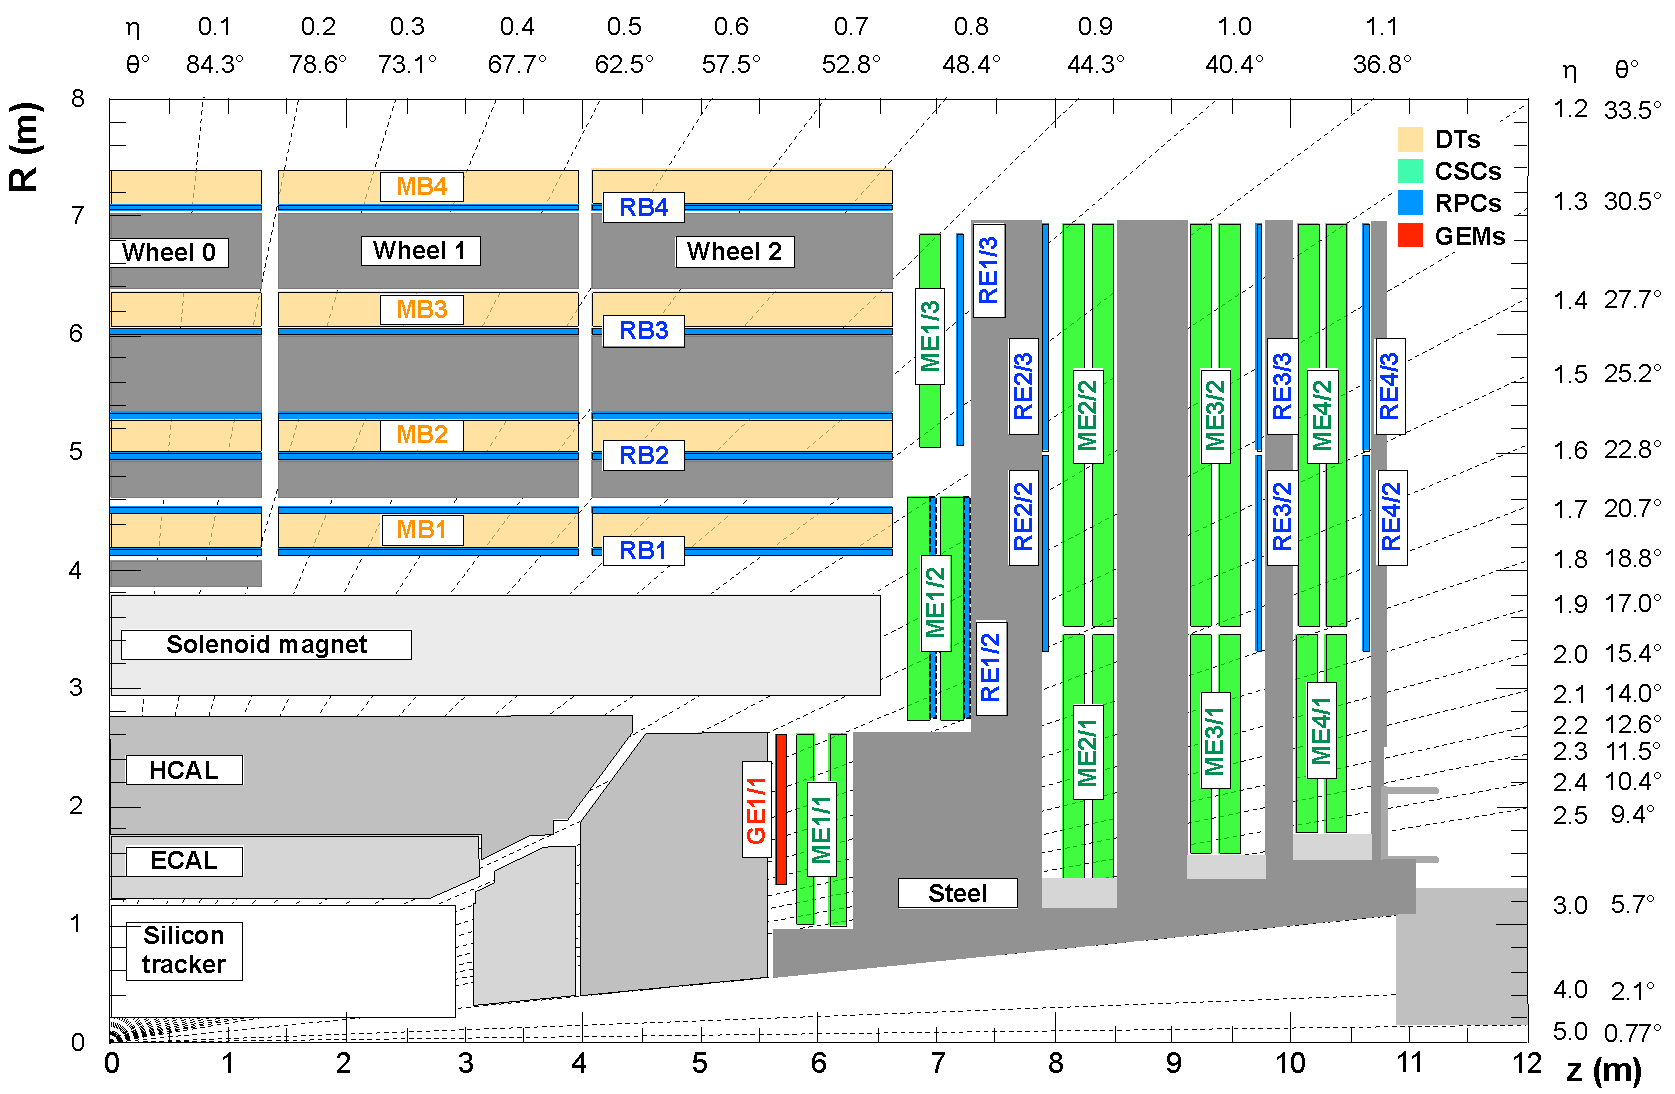
\includegraphics[width=0.95\textwidth]{figures/GEM/cms_upg_o_g_b_ni_ge1_r_140227.pdf}
    \caption{A cross-sectional view of the CMS quadrant highlighting the location of GEM detectors (red).}
    \label{fig:GE1/1pos}
\end{figure}

\subsection{CMS GE1/1 Detector Specification} % (fold)
\label{sub:GE1/1_detector_details}
A typical GE1/1 detector is trapezoidal in shape with an active area of $990~\times~(220-445)~mm^2$.
The shape and size fo the detector was decided based on the geometry of vacant high-$\eta$ region in the CMS muon endcap regions.
A GE1/1 chamber consists of a Triple-GEM detector having a $3/1/2/1~mm$ (drift/transfer 1/transfer 2/induction) electrode gap configuration, as shown in Fig. \ref{fig:tripple-gem}.
\begin{figure}[!htbp]
    \begin{center}
        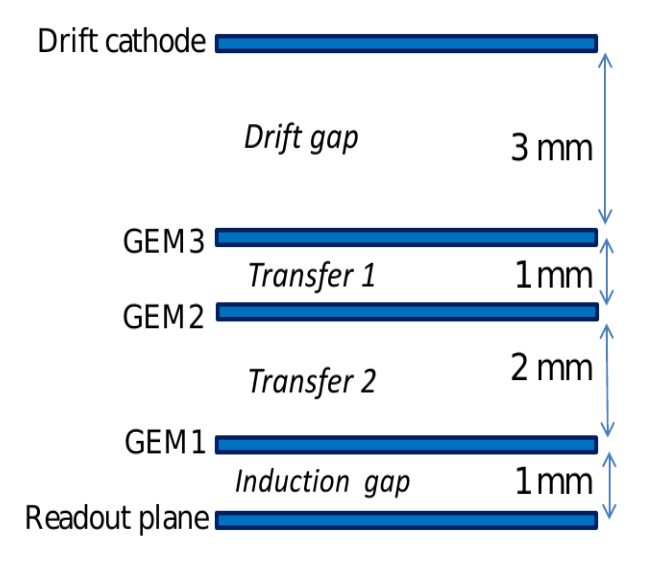
\includegraphics[width=0.45\textwidth]{figures/GEM/tripple-gem.png}
        \caption{The layout of different GEM layers inside a CMS GE1/1 detector.}
        \label{fig:tripple-gem}
    \end{center}
\end{figure} 
% ($50~\mu m$ thick Kapton foil with $5\mu m$ copper on both sides) 
The GEM foil consists of a thin Kapton foil ($50~\mu m$ thick) with a copper clad ($5~\mu m$) on both sides.
The detector readout board is divided into eight $\eta$-partitions with 384 strips.
Each strip is radially oriented along the long side of the detector with a pitch varying from $0.6~mm$ (short side) to $1.2~mm$ (long side).
Each partition is subdivided along the $\phi$-coordinate into three readout sectors with 128 strips or channels per sector. The $\eta$ partition and $\phi$ portions of the GEM detector are shown in Fig.~\ref{fig:gemTrapezoidal}.
\begin{figure}[!htbp]
    \begin{center}
        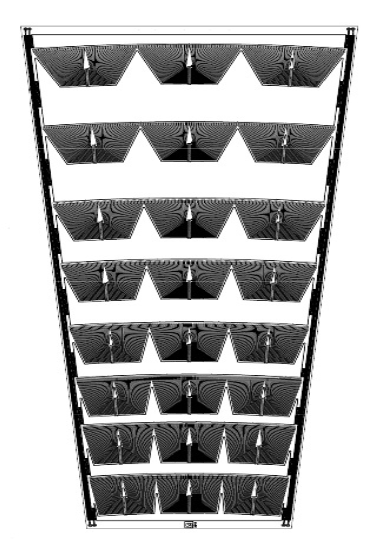
\includegraphics[angle=-90,width=0.75\textwidth]{figures/GEM/gemTrapezoidal.png}
        \caption{Drawing of a large trapezoidal CMS GEM chamber showing $8-\eta$ and $3-\phi$ par partitions.}
        \label{fig:gemTrapezoidal}
    \end{center}
\end{figure} 
To improve tracking capabilities, two GEM chambers will be mounted face-to-face to form a double layer called ``\textit{Super-Chamber}".
Thus each Super-Chamber will provide two impact points for each muon track.
The full layer by layer mechanical design of a GEM chamber is shown in Fig.~\ref{fig:GE1/1}. 
The main parts in a GEM detector are GEM foil, drift plane, readout board, shielding, high voltage divider, etc.
\begin{figure}[!htbp]
    \begin{center}
        \includegraphics[width=0.95\textwidth]{figures/GEM/GE11cad.png}
        \caption{Layer by layer view of GEM detector}
        \label{fig:GE1/1}
    \end{center}
\end{figure} 
\todo[inline]{Add a para on fig~\ref{fig:GE1/1}}
\todo[inline]{Add a para on GE1/1 fabrication}
% \begin{figure}[!htbp]
% \centering
% 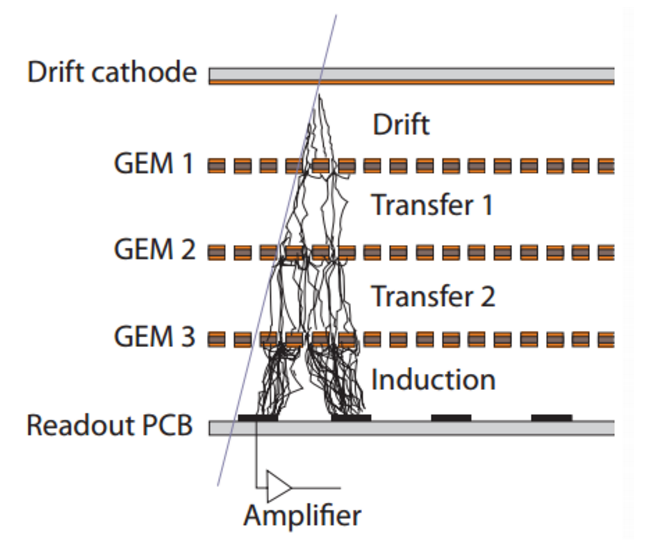
\includegraphics[width=2.0in]{figures/GEM/GEMCascade.png}
% \caption{Generic triple-GEM chamber, showing drift, transfer, and signal induction gap regions within the detector.}
% \label{GEM:cascade}
% \end{figure}

\subsection{GE1/1 Beam Test Studies}
The GE1/1 detector was tested using 150 GeV muon and pion beams at CERN SPS beam test facility during October-December 2014. 
The goal of the beam test campaign was to measure the efficiency, space \& time resolution, and the cluster size of the CMS GEM detector. 
The detectors that were tested includes GE11\_IV\_CERN\_0001 and GE11\_IV\_CERN\_0002 detectors(detectors naming convention and its details are mentioned in the appendix~\ref{cha:GE1/1_detector_generations}).
Two beam test campaign was carried out during October-December 2014.
These campaign held in H2 and H4 beam test area of CERN SPS.
The H2 beam test was held from $6^{th}$ October 2014 to $27^{th}$ October 2014 while the H4 beam test was held from 26 November to 14 December 2014.
The main goal of the H2 beam test was to test the two detectors mentioned above with an $Ar:CO_2$ gas mixture while in H4 beam test the same detector was tested with $Ar:CO_2:CF_4$ gas mixture.
Initially, the plan was to scan each sector of the GEM detectors but due to timing constraints we were just able to scan sector $(i\eta, i\phi)=\{(5,2)\}$ and $(i\eta,i\phi)=\{(1,2),(5,2),(8,2)\}$ during H2 and H4 beam test respectively.  

The data collected during these beam test campaigns were grouped into different run names, based on the electronic setup and gas mixtures used during the data taking. Out of these four set of run ranges were marked as ``\textit{good}'', based on certain data quality checks, for further analysis. These run ranges along with their specification are listed in Table~\ref{tab:gemTBgoldenruns}

\begin{table}
\begin{tabular}[!htbp]{l l}
\hline
\textbf{Run Name}   &   \textbf{Details}\\
\hline
2014H2C     & Run range: 306-407    \\
            & Threshold for each VFAT strip = 15 VFAT units\footnote{1 VFAT unit = 0.08 fC} = 1.2fC\\
            & Asynchronous mode with respect to the LHC clock \\
            & sector scanned $(i\eta, i\phi)=(5,2)$\\
            & Gas mixture used: $Ar:CO_{2}$=(70:30)\\
\hline
2014H4A     & Run range: 1592-1646 \\
            & Threshold for each VFAT strip = 15 VFAT units = 1.2fC\\
            & Asynchronous mode with respect to the LHC clock \\
            & sector scanned $(i\eta, i\phi)=(5,2)$\\
            & Gas mixture used: $Ar:CO_{2}:CF_4$=(40:15:45)\\
\hline
2014H4C     & Run range: 1868-1906 \\
            & Threshold for each VFAT strip = 15 VFAT units = 1.2fC\\
            & Asynchronous mode with respect to the LHC clock \\
            & sector scanned $(i\eta, i\phi)=(8,2)$\\
            & Gas mixture used: $Ar:CO_{2}:CF_4$=(40:15:45)\\
\hline
2014H4D     & Run range: 2065-2123 \\
            & Threshold for each VFAT strip = 15 VFAT units = 1.2fC\\
            & Asynchronous mode with respect to the LHC clock \\
            & sector scanned $(i\eta, i\phi)=(1,2)$\\             
            & Gas mixture used: $Ar:CO_{2}:CF_4$=(40:15:45)\\
\hline
\end{tabular}
\caption{List of golden runs used to measure the GE1/1 properties.}
\label{tab:gemTBgoldenruns}
\end{table}
% subsection GE1/1_detector_details (end)
\subsubsection{Information on GEM detectors used in the beam test} % (fold)
\label{ssub:information_of_gem_detectors_used_in_test_beam}
The two detectors used in the beam test are GE11\_IV\_CERN\_0001 and \\GE11\_IV\_CERN\_0002. 
Both GE11\_IV\_CERN\_0001 and GE1/1\_IV\_CERN\_0002 are generation IV GE1/1 detectors but GE1/1\_IV\_CERN\_0002 was irradiated with the gamma-ray at the CERN gamma-ray irradiation facility for 1 year to perform ageing studies~\cite{Merlin2013}. 
The high voltage configuration used during the beam test is shown in Fig.~\ref{fig:HV_configuration}. 
Also, the voltage across the GEM foils and  the electric field  with respect to the current in the voltage divider is shown in Fig.~\ref{fig:GEM_voltage_electricfield}. 
The gain of the detector was measured in the lab using an X-ray source for both $Ar:CO_2$ and
 % is shown in Fig.~\ref{fig:gain_GE1/1_IV} and with gas 
 $Ar:CO_2:CF_4$ gas mixture and is shown in Fig.~\ref{fig:gain_GE1/1_IV_GIF} and ~\ref{fig:gain_GE1/1_IV}. 
The gain of a detector can be calculated using the ratio of output to the input value of current, like:
\begin{equation}
    Gain~=~\frac{I_{out}}{q~\times~f}
\end{equation}
where q is the charge collected at the first layer of GEM foil and is calculated as:
\begin{equation}
    q~= n~\times~e
\end{equation}
where e is the electron charge, n is the average number of electrons produced in the drift region by the incident particles and $f$ is the interaction rate of the incident particles in the gas. For the given X-ray source with a specific energy and the known ionization potential of the used gas mixture n can be calculated and is found to be $n \sim 290$.
\begin{figure}[htbp]
    \centering
    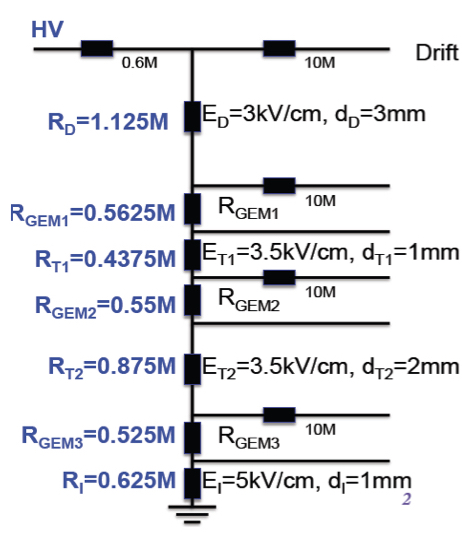
\includegraphics[width=0.40\textwidth]{figures/GEM/HV_divider_gem_testbeam_2014.jpeg}
    \caption{High voltage divider configuration as used in the 2014 beam test campaign.}
    \label{fig:HV_configuration}
\end{figure}
\begin{figure}[htbp]
    \centering
    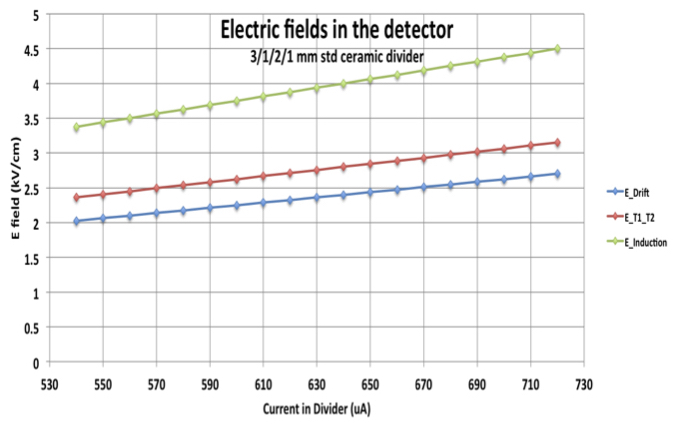
\includegraphics[width=0.5\textwidth]{figures/GEM/GE11_IV_ElectricField_detector.jpeg}%
    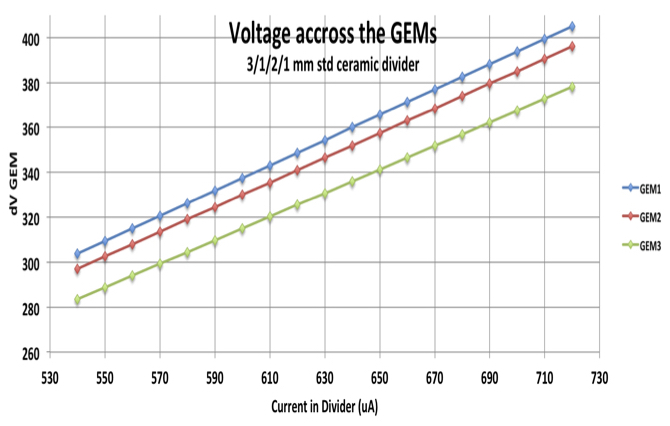
\includegraphics[width=0.5\textwidth]{figures/GEM/GE11_IV_VoltageAcross_GEM.jpeg}
    \caption{Electric field (left) and voltage across each GEM foil (right) for the tested GE1/1 detector.}
    \label{fig:GEM_voltage_electricfield}
\end{figure}
\begin{figure}[htbp]
    \centering
    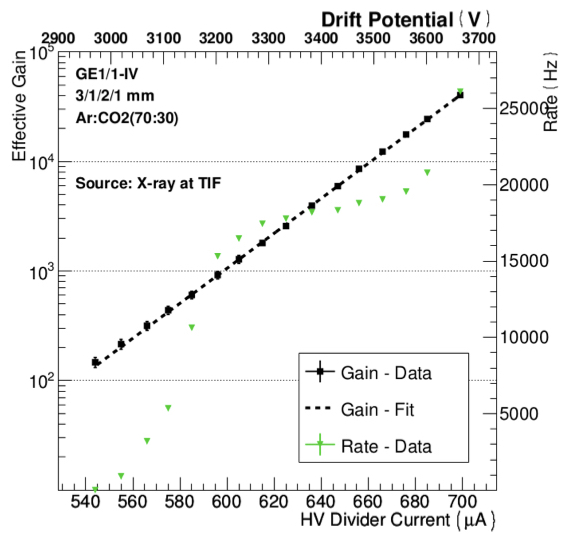
\includegraphics[width=0.5\textwidth]{figures/GEM/Gain_curve_GE11_IV_Ar_CO2.jpeg}%
    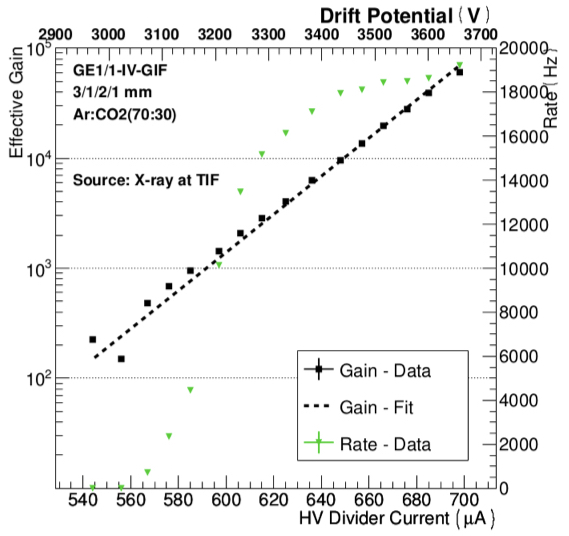
\includegraphics[width=0.5\textwidth]{figures/GEM/Gain_curve_GE11_IV_GIF_Ar_CO2.jpeg}
    \caption{Gain and rate variation for $Ar:CO_2$ (70:30) with respect to the current supplied to the high voltage divider for GE1/1-IV (left) and GE1/1-IV-GIF (right).}
    \label{fig:gain_GE1/1_IV}
\end{figure}
\begin{figure}[htbp]
    \centering
    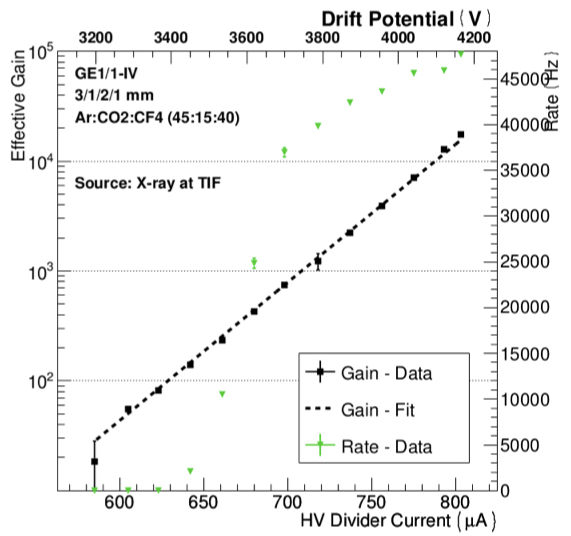
\includegraphics[width=0.5\textwidth]{figures/GEM/Gain_curve_GE11_IV_Ar_CO2_CF4.jpeg}%
    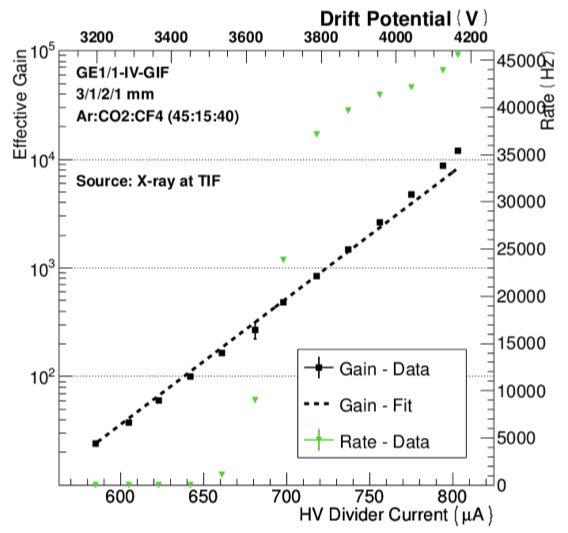
\includegraphics[width=0.5\textwidth]{figures/GEM/Gain_curve_GE11_IV_GIF_Ar_CO2_CF4.jpeg}
    \caption{Gain and rate variation for $Ar:CO_2:CF_4$ (45:15:40) with respect to the current supplied to the high voltage divider for GE1/1-IV (left) and GE1/1-IV-GIF (right).}
    \label{fig:gain_GE1/1_IV_GIF}
\end{figure}
% subsubsection _information_of_gem_detectors_used_in_test_beam (end)

\subsubsection{Readout Electronics} % (fold)
\label{ssub:readout_electronics}
Front-end electronics used in the beam test was \textbf{\textit{VFAT2}} chips~\cite{Aspell2007,Berardi2004}.
The upgraded version of the same chip, known as VFAT3, will be used with CMS GE1/1 detectors for Level-1 muon triggering~\cite{Licciulli2017}. Its block diagram is shown in Fig.~\ref{fig:VFAT2block}.

VFAT is a front-end Application Specific Integrated Circuit (ASIC) chip was primarily designed for the readout of sensors in the TOTEM experiment at CERN. 
VFAT chip is used for both triggering and tracking purpose.
For triggering it uses the programmable ``\textit{fast OR}'' information based on a hit in the detector.
It provides a monostable output for the programmed number of channels in a single clock cycle. 
This is called an ``S-Bit''. While, for tracking it provides the spatial information strip-wise for every triggered event.

VFAT2 has 128 analog input channels, very low noise pre-amplifier, shaper and comparator attached to it. 
Signal discrimination is done based on the programmable threshold setting and then stored within SRAM\footnote{Static random-access memory (static RAM or SRAM) is a type of semiconductor memory that uses bistable latching circuitry (flip-flop) to store each bit. SRAM exhibits data remanence but it is still volatile in the conventional sense that data is eventually lost when the memory is not powered.} until the trigger information is received. 
It can apply positive as well as negative threshold value to each channel independently. 
This feature is named as ``\textit{TrimDAC}'' and the VFAT chip has two programmable voltages $V_{T1}$ and $V_{T2}$ and the threshold is defined as the difference between these two programmable voltages, i.e., $V_{TH} = V_{T2} - V_{T1}$.

This VFAT chip also provides the facility to mask individual noisy channel.

To synchronize the output of the comparator the monostable block provides 1 clock pulse for each threshold-crossing signal.

\begin{figure}[htbp]
    \centering
    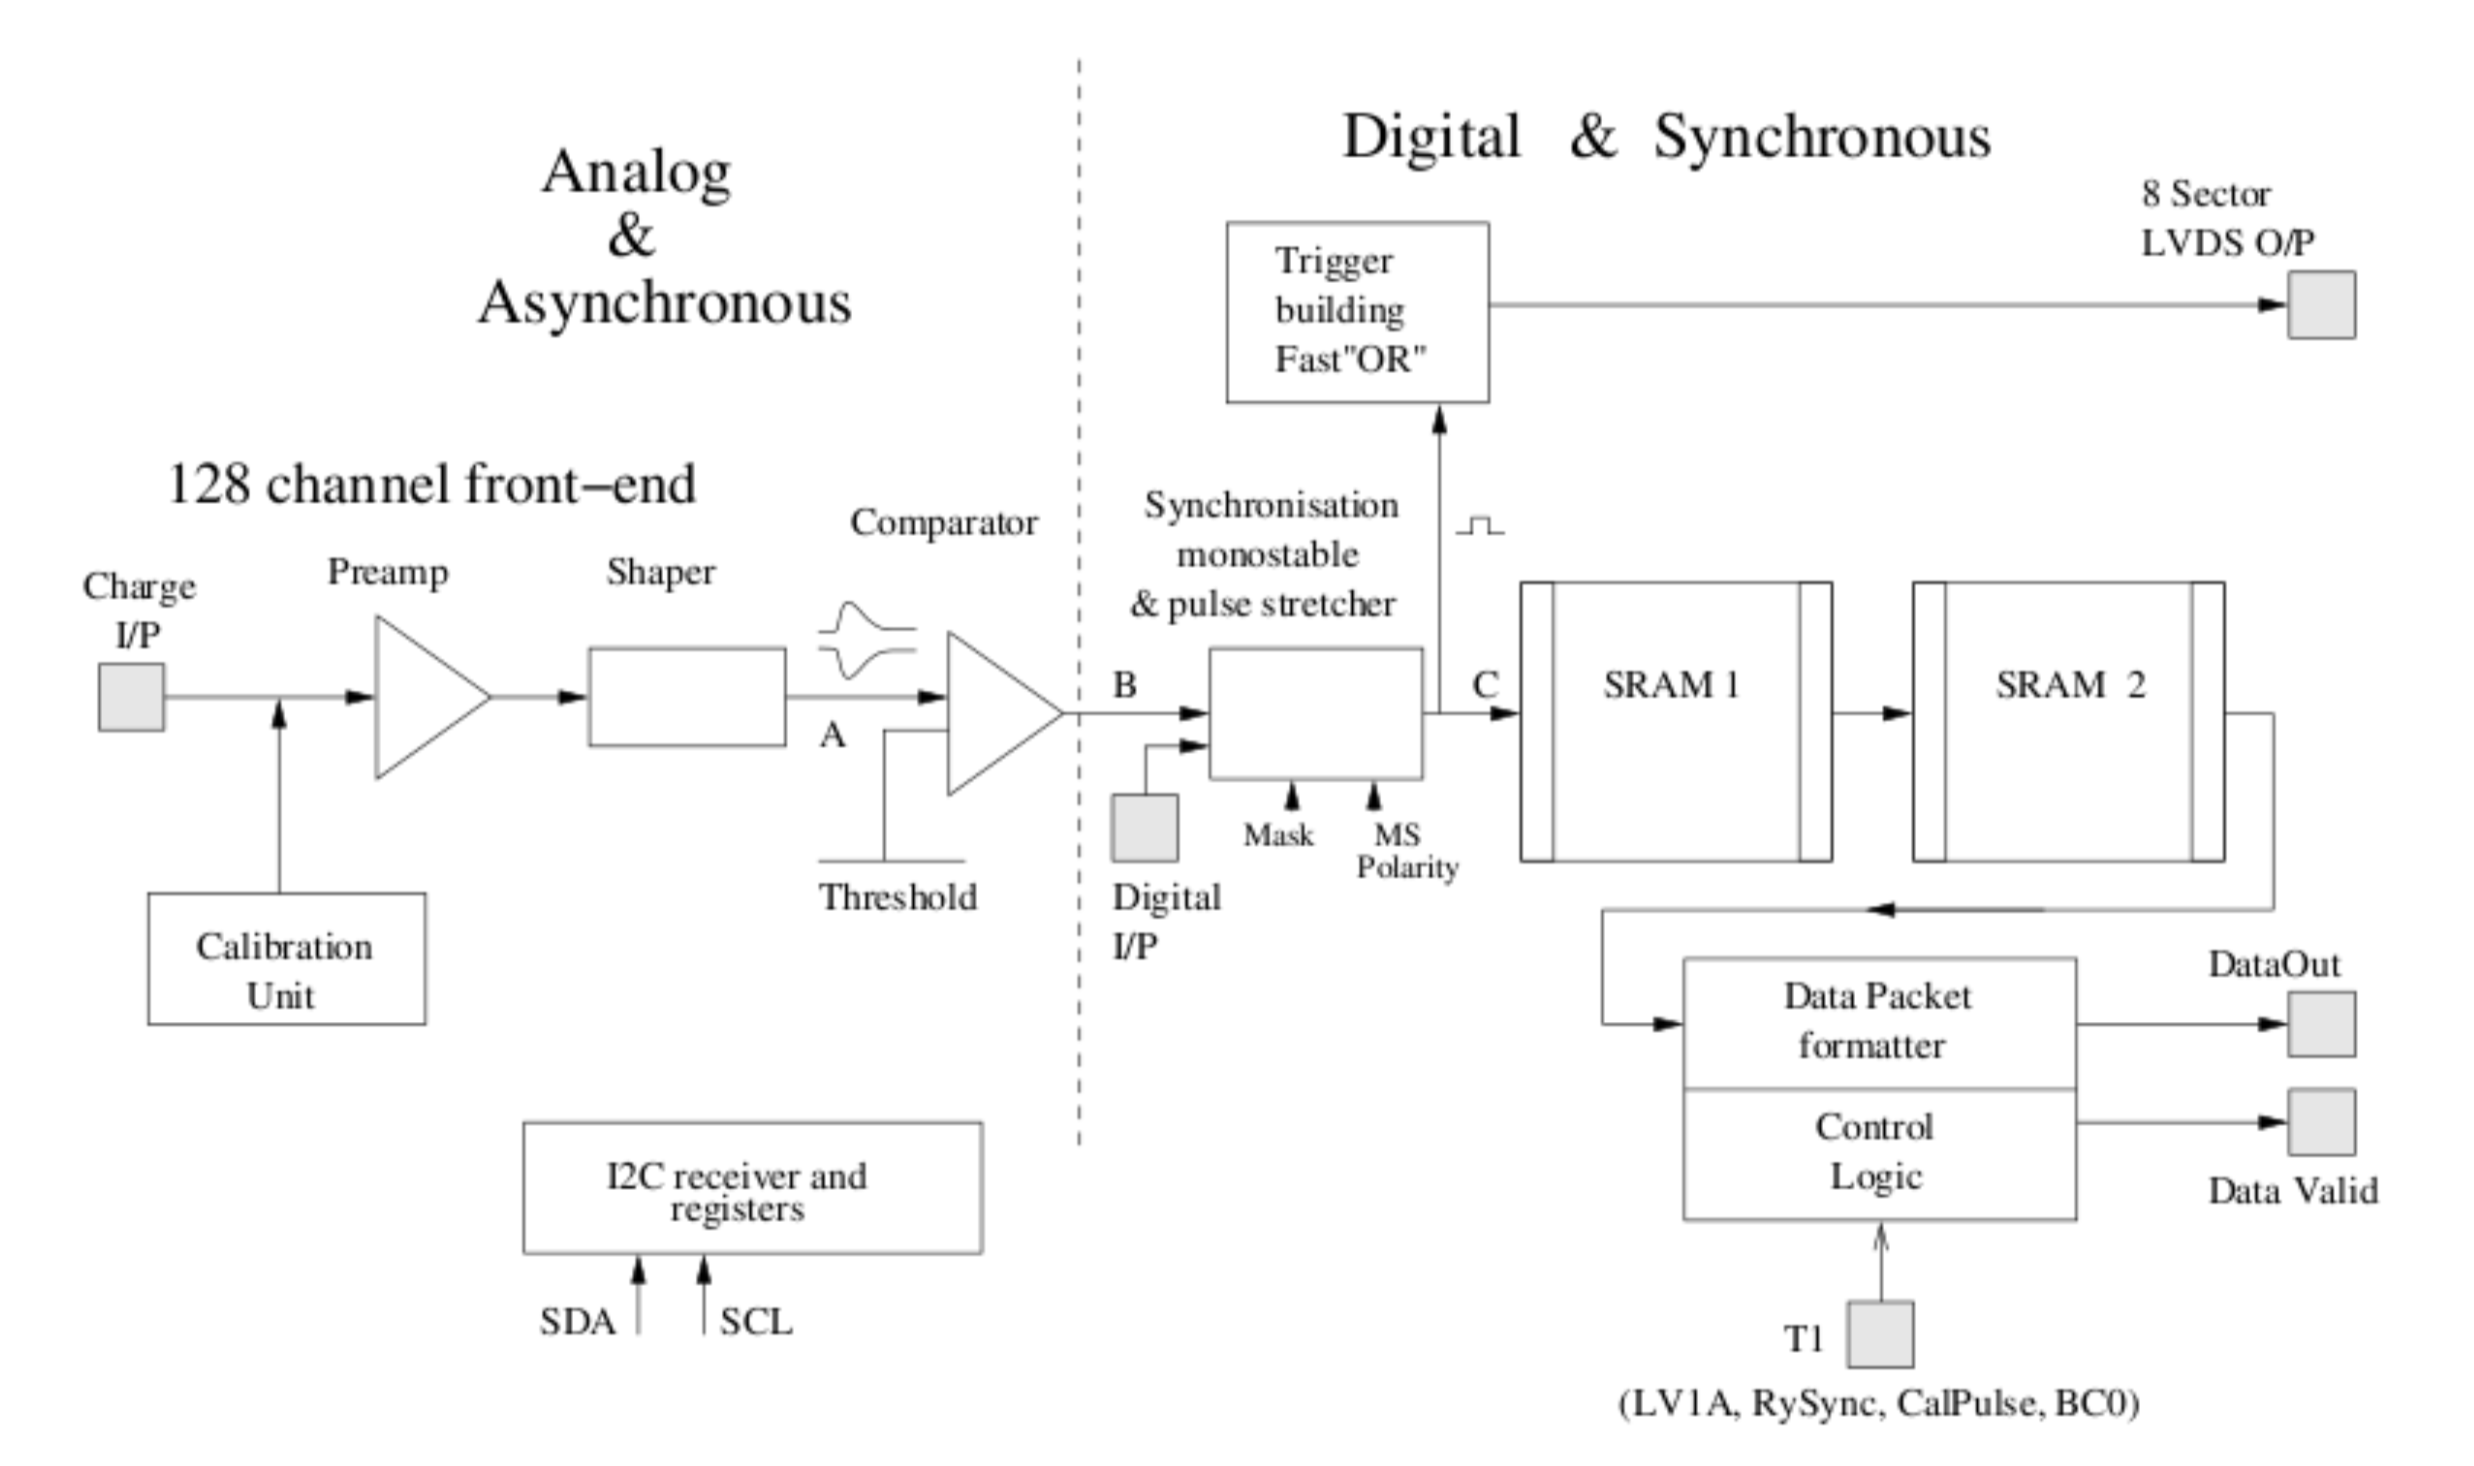
\includegraphics[width=0.95\textwidth]{figures/GEM/VFAT2_chip_BlockDiagram.png}
    \caption{Block diagram of the VFAT2 chip showing signal flow~\cite{Aspell2007}.}
    \label{fig:VFAT2block}
\end{figure}



\textbf{Latency} defines the correct moment of time at which VFAT2 will read the signal. Technically, for a given trigger, it is defined as the number of SRAM locations the chip has to go back in order to read the digital output of the event corresponding to that trigger. It is measured in clock periods. 

% \textbf{Monostable settings}

\subsubsection{TURBO Readout Board} % (fold)
\label{ssub:turbo_readout_board}
TURBO is a standalone DAQ system for the VFAT front-end ASIC~\cite{Paschalis2011}. It was developed for testing TOTEM hybrid equipped with VFAT chips, with following goals:
\begin{itemize}
    \item portable,
    \item real-time response,
    \item DAQ capability for small and medium-sized experiments.
\end{itemize}
\begin{figure}[htbp]
    \centering
    \includegraphics[width=0.75\textwidth]{figures/GEM/TRUBO_testbam_labelled.png}
    \caption{TURBO board~\cite{Paschalis2011}.}
    \label{fig:turbo}
\end{figure}
Each TURBO can accommodate up to 8 VFAT chips. 
A systematic diagram of TURBO board is shown in Fig.~\ref{fig:turbo}. 
But, one can use more than 1 TURBO boards to accommodate more than 8 VFAT chips. 
Out of them, one TURBO board will act as the master board that will take care of the clock for other TURBO boards, which act as slaves.

A LabView program can be used to control TURBO boards remotely. 
This program can perform standard calibration scans such as threshold and latency scans as well as can be used for data acquisition and quality control tests.
% subsubsection turbo_readout_board (end)

% subsubsection readout_electronics (end)

\subsubsection{Measurement Mode} % (fold)
\label{ssub:measurement_mode}
Data can be collected in two different modes: synchronous mode and asynchronous mode. In the asynchronous mode, triggers are not correlated with the clock while in a synchronous mode triggers are correlated with the leading edge of the clock. Synchronous mode is used to collect data in sync with the LHC clock.
% subsubsection measurement_mode (end)

\subsection{Beam Test Experimental Set-up}
% A simple schematic diagram of the experimental setup is shown in Fig.~\ref{fig:tbsetup}.
The experimental set-up consists of three plastic organic scintillators, three trackers and a GE1/1 prototype, being flushed with an Ar/CO$_{2}$ (70:30) gas mixture.
The trackers are triple-GEM detectors having an active area of $10~cm\times10~cm$ having 256 strips in both horizontal (y-coordinate) and vertical (x-coordinate) directions with respect to the beam and a pitch of $0.4~mm$.
The three trackers constitute a muon tracking telescope which is used to reconstruct the beam trajectories and reduce background events.
Figure~\ref{fig:tbs} shows the experimental set-up used to perform beam test studies.
The GE1/1 prototypes are installed on a movable table to scan different sectors. At a time only one (i$\eta$,i$\phi$) sector of GEM detector is irradiated with the beam.
% The high voltage powering was realized using a ceramic high voltage divider. 
The CMS test chamber was placed, close to the tracking hodoscope, on a vertically movable support to allow scanning. The scanned sectors of the GE1/1 detector are shown in Fig.~\ref{GE1/1}.

The tracking telescope is equipped with the digital chips VFAT2~\cite{Aspell:2008zz}, which provides a binary output with a variable latency for the position information and a fixed latency output, called SBIT, for the timing information.

% \begin{figure}[!htbp]
%     \begin{center}
%         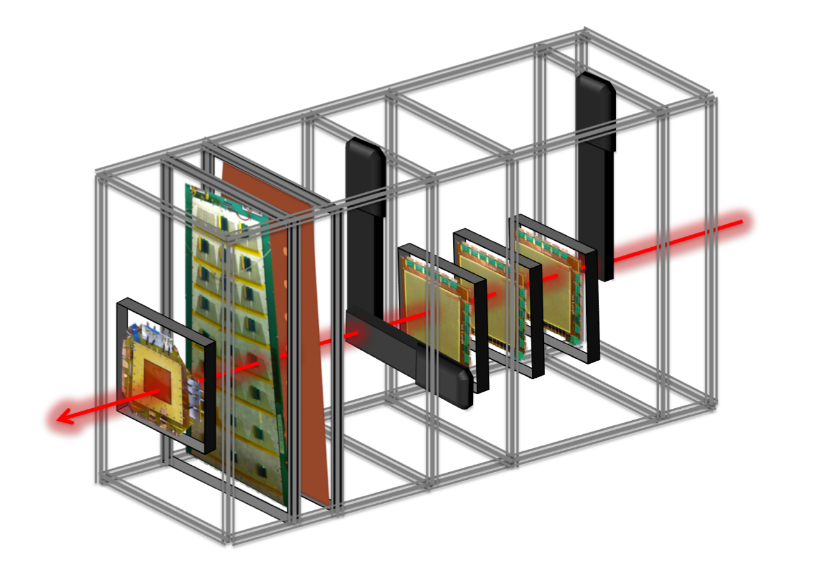
\includegraphics[width=0.95\textwidth]{figures/GEM/tbsetup.png}
%         \caption{Schematic view of the beam test set-up with the three square GEM hodoscope and the trapezoidal CMS GEM chambers}
%         \label{fig:tbsetup}
%     \end{center}
% \end{figure} 
\begin{figure}[!htbp]
\centering
% 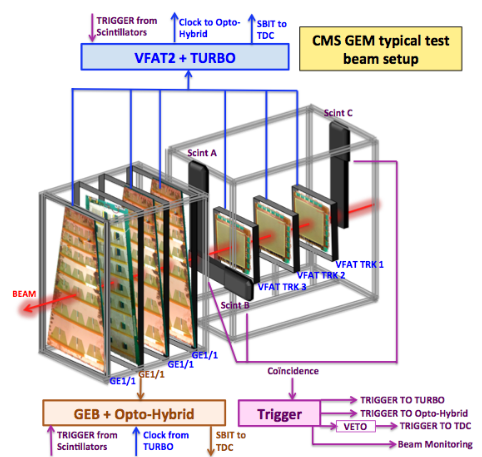
\includegraphics[width=0.95\textwidth]{figures/GEM/tb_exptsetup.png}
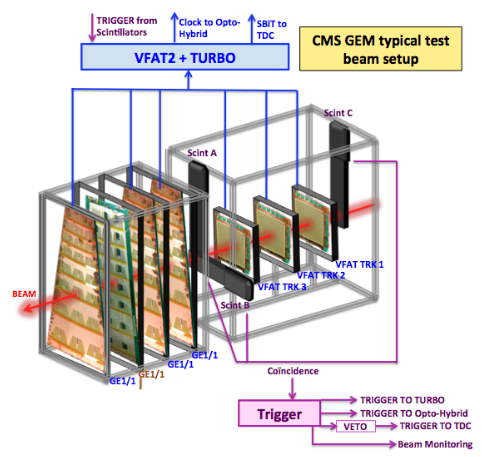
\includegraphics[width=0.75\textwidth]{figures/GEM/tb_exptsetup_copy.png}
\caption{Schematic view of the beam test set-up with the three tracking GEM detectors and a GE1/1 prototype.}\label{fig:daq}
\end{figure}
On detector electronics connects the output from the front-end ASIC (VFAT2) to the GEM readout board.
The VFAT2 chip is connected to the hybrids which are plugged into the connectors on the readout board.
%The trigger is generated using the coincidence of three photo-multiplier tubes with mounted scintillators. 
The analog pulses from the three scintillators, named S1, S2 and S3 are fed into discriminator for analog to digital conversion.
The discriminator output was provided into the logic coincidence (to generate event trigger) before being sent to the other DAQ systems (Figure.~\ref{fig:daq}).
\begin{figure}[!htbp]
\centering
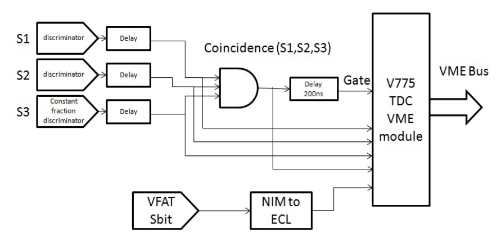
\includegraphics[width=0.95\textwidth]{figures/GEM/daq.png}
\caption{Perspective view of the experimental set-up used for performance measurement in the beam test studies. The trigger system is generated using the signal collected from three scintillators connected in coincidence.}\label{fig:tbs}
\end{figure}
The active area of the GE1/1 detector is covered with readout strips located in the GEM Electronic Board. 
The readout strips are taken out in 24 readout sectors (in ($\eta$,$\phi$) phase space).
The data from each sector are collected using a VFAT2 front-end chip. 


%, with a tracker pitch of $0.4~mm$
\begin{figure}[!htbp]
\centering
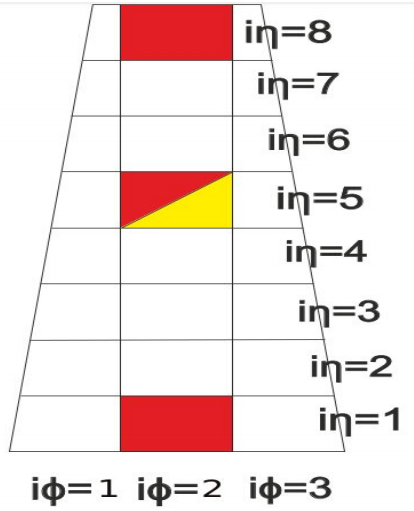
\includegraphics[scale=0.5,angle=90]{figures/GEM/GE11.png}
\caption{Different $(i\eta,i\phi)$ sectors of a full-size GE1/1 detector prototype. The red and yellow colour shows which sector of GE1/1 is exposed to the beam. Red sectors are collected with $Ar/CO_2/CF_4~(45/15/40)$ gas mixture while the yellow sectors are taken with $Ar/CO_2~(70/30)$ gas mixture.}
\label{GE1/1}
% THis is for beam test
\end{figure}
\subsection{Data Analysis} % (fold)
\label{sub:test_beam_analysis}
The raw data collected during these beam test campaign were in binary format. First, the raw data (binary information) is converted into the ROOT data format. ``\textit{\textbf{TURBO-SOFTWARE}}''~\cite{git-trubosoftware} package is used for data analysis framework, originally developed by TOTEM group, is used to perform this task. The output from TURBO-SOFTWARE data analysis consists of hit information from the detectors which are further used to reconstruct the particle tracks and clusters. 

A \textbf{hit} is defined when one or more strip of the VFAT chips surpass the threshold set on the readout chip. 
A \textbf{cluster} is defined as the number of adjacent fired strips along x or y-axis. The first step towards the track and cluster reconstruction is to discriminate the background tracks coming from detector noise (fake tracks) from the signal (muon) tracks. Once the fake tracks are removed from the collection, valid hits are used to generate tracks.

The hit profile and beam profile recorded in the tracker for one of the run are shown in Fig.~\ref{HitPosXaxis}~and~\ref{BeamProfile}.
From both hit profile and beam profile, one can see that the beam is point beam like a beam having a Gaussian spread, centred around (50,50), i.e., at the centre of the tracker.

This sorting is done by selecting events having only one cluster in each tracker. Then, the cluster positions are fitted using a polynomial fit of order one and $\chi^2$ of the fit is recorded.
The event is discarded if the $\chi^2$ of the fit is greater than 10.
\begin{figure}[!htbp]
\centering
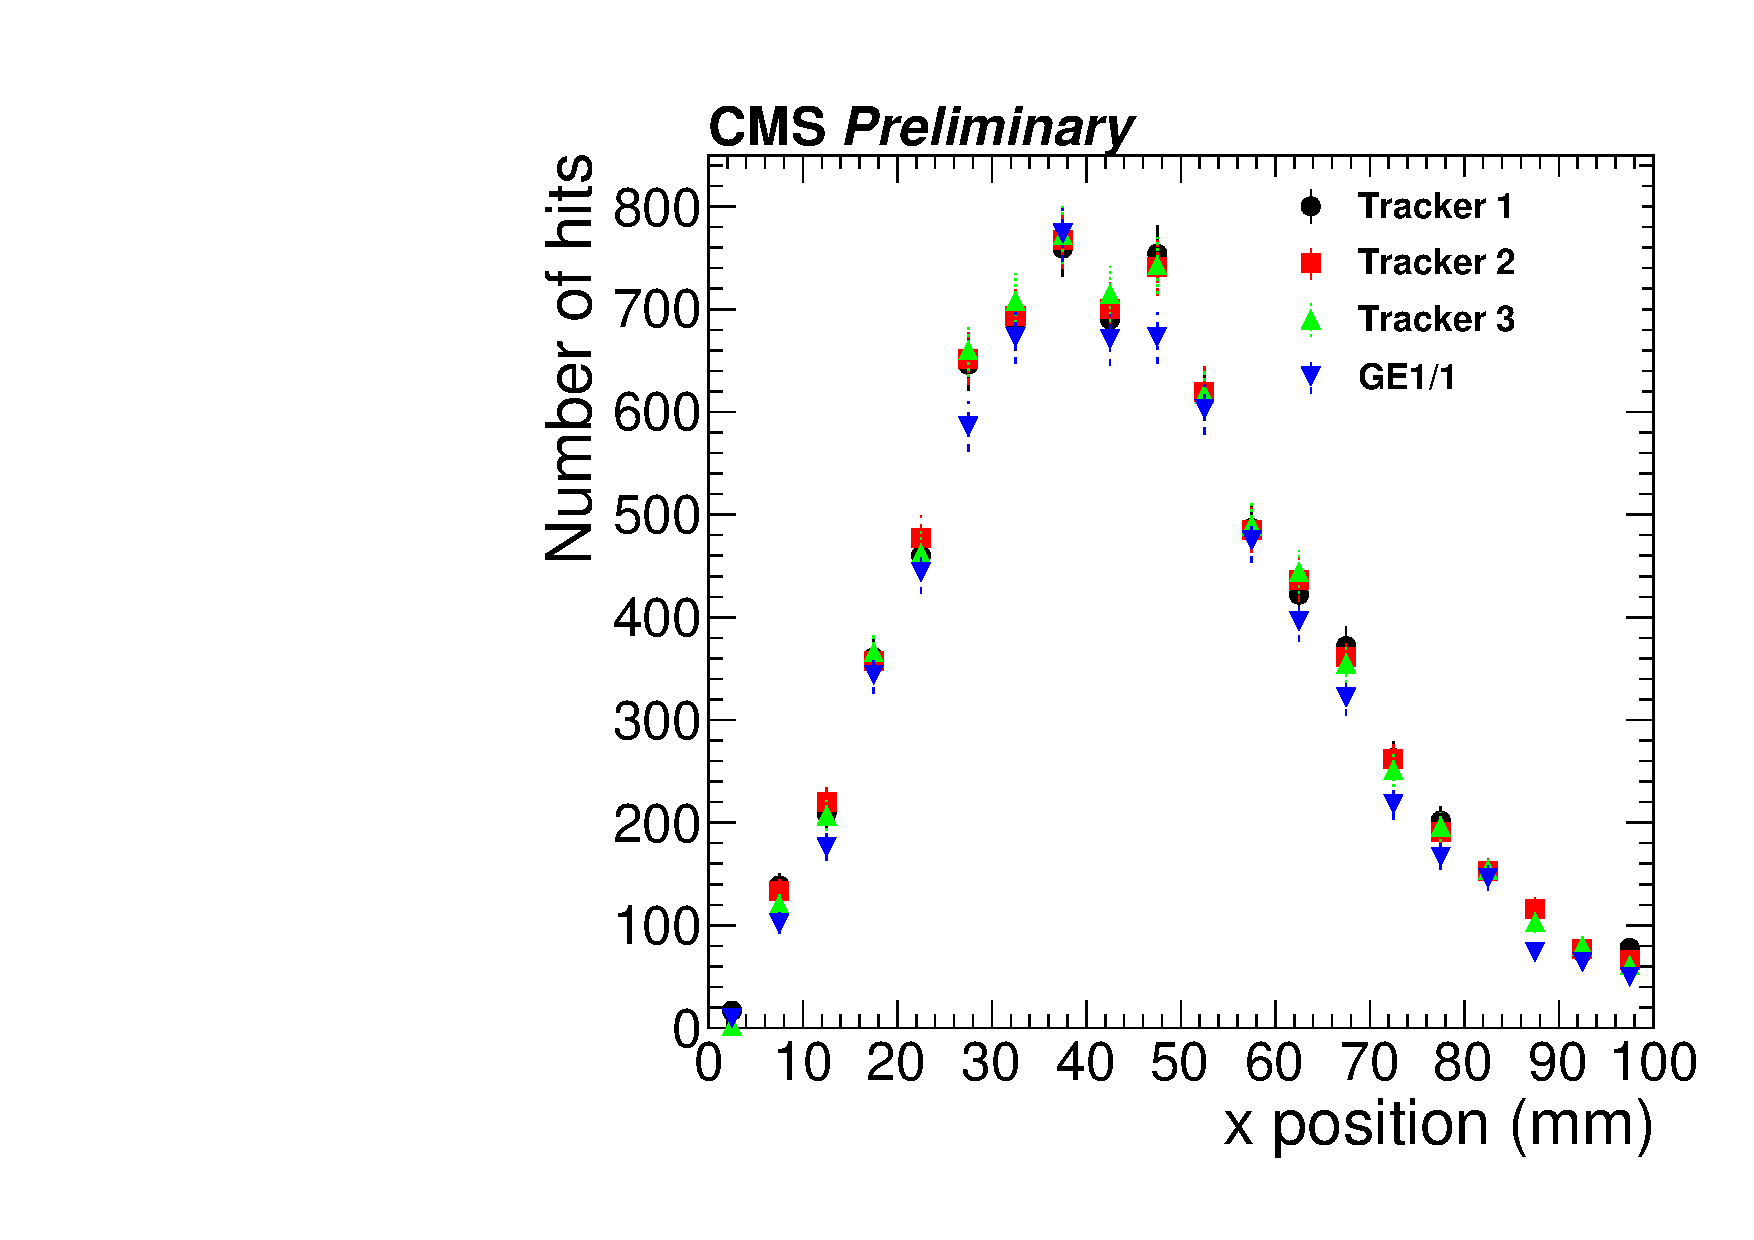
\includegraphics[width=0.45\textwidth]{figures/GEM/Tracker_Hit_position_Run1644_x.pdf}%
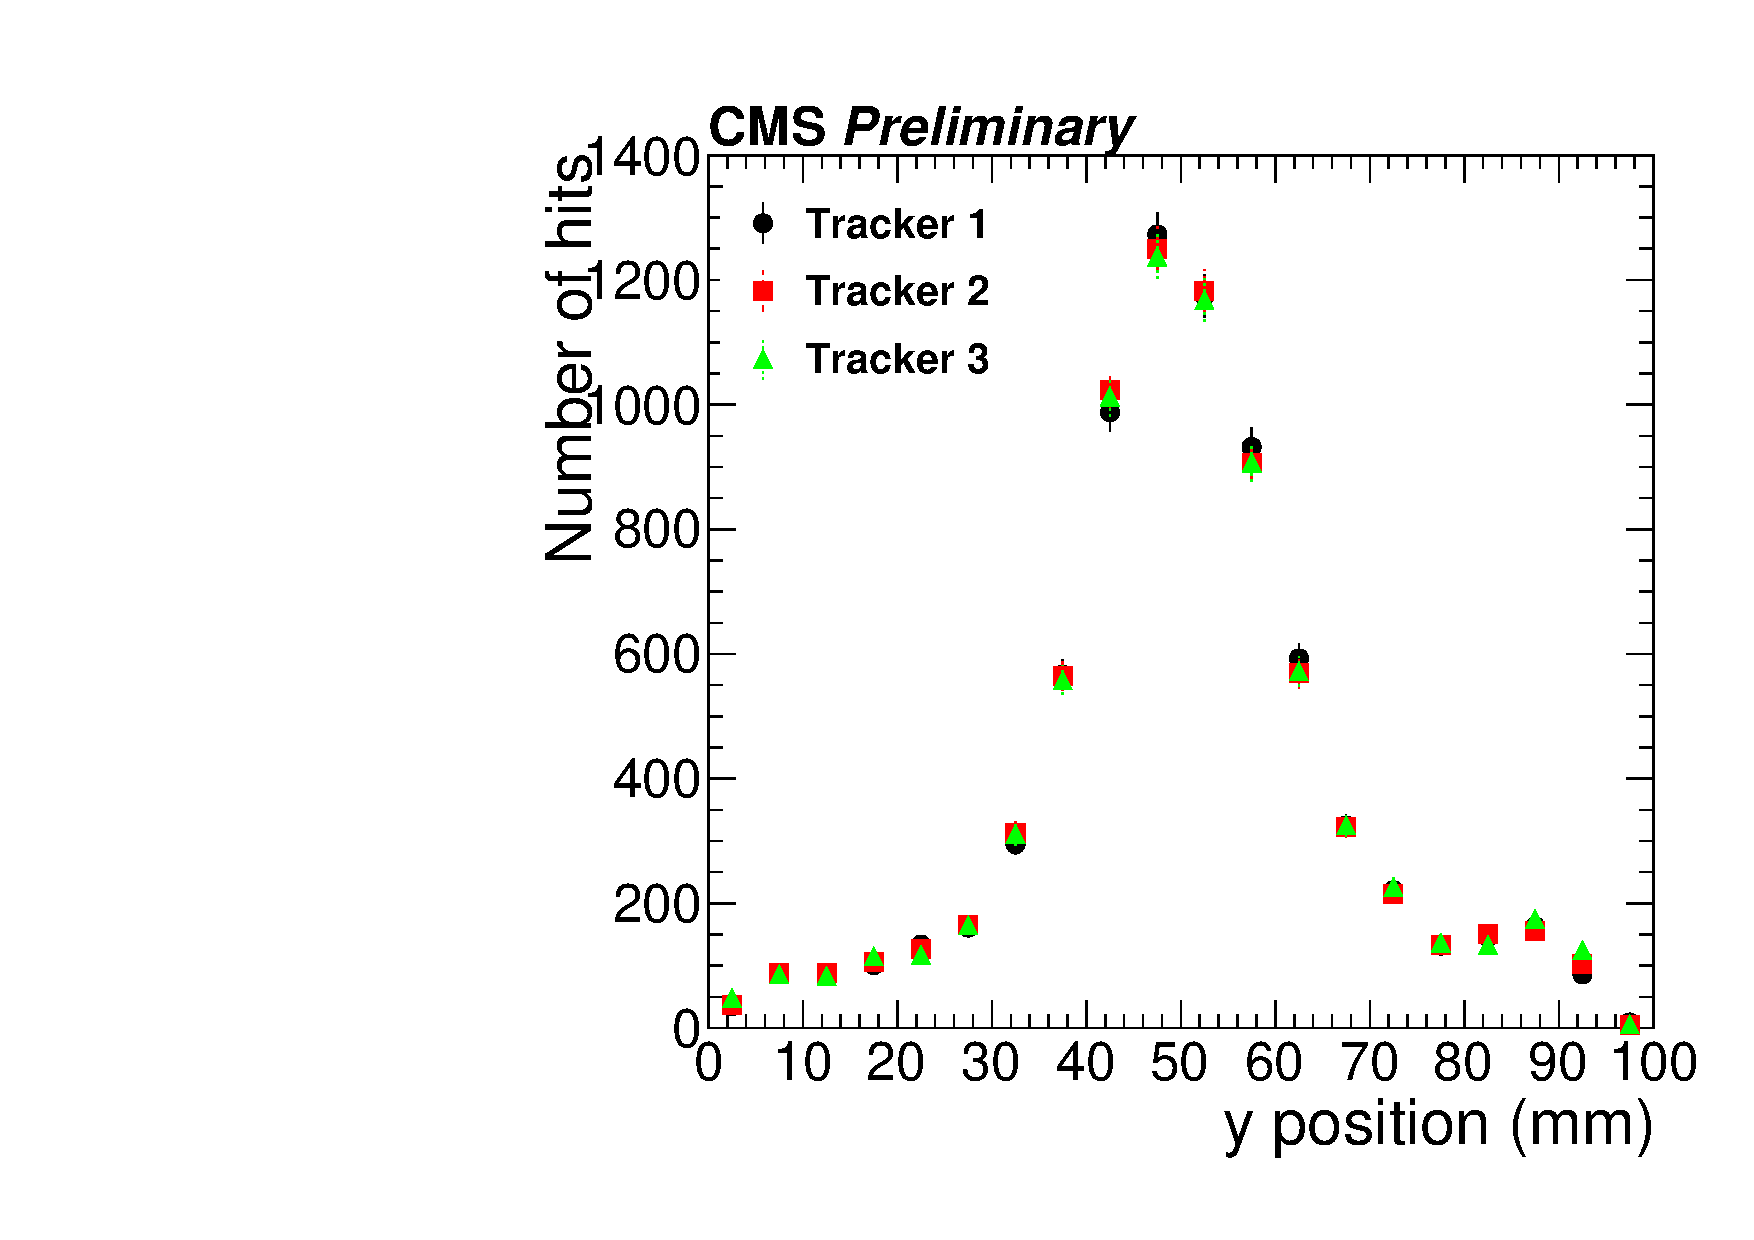
\includegraphics[width=0.45\textwidth]{figures/GEM/Tracker_Hit_position_Run1644_y.pdf}
\caption{Tracker hit distribution along x and y axis and GE1/1 hit distribution along y. This is plotted from one of run taken during test-beam.}
\label{HitPosXaxis}
\end{figure}
\begin{figure}[!htbp]
\centering
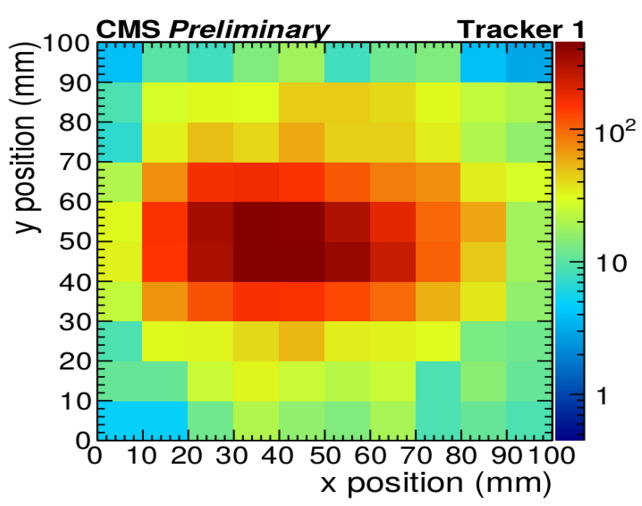
\includegraphics[width=0.5\textwidth]{figures/GEM/Selection_027.png}%
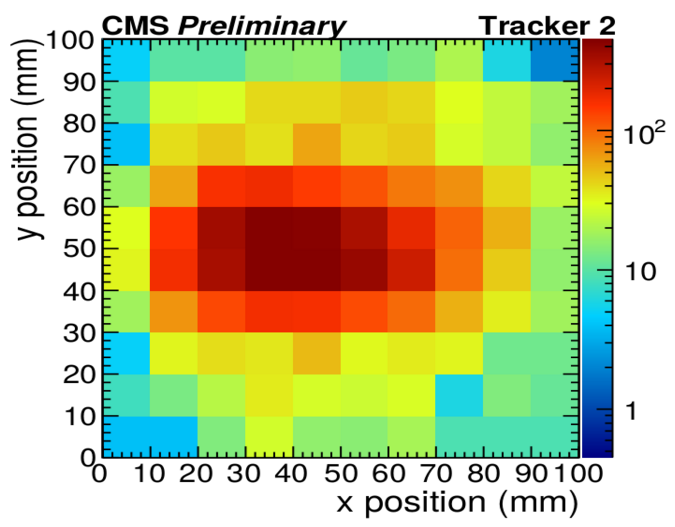
\includegraphics[width=0.5\textwidth]{figures/GEM/Selection_028.png}\\
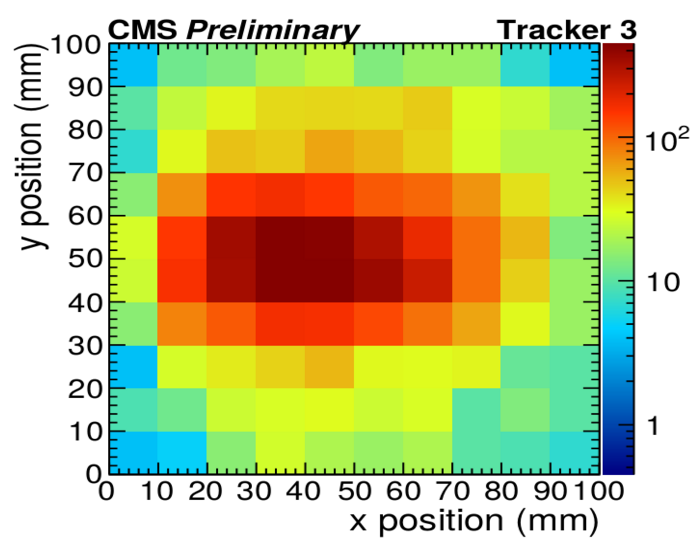
\includegraphics[width=0.5\textwidth]{figures/GEM/Selection_029.png}
\caption{2D- beam profile plot for the first, second and third tracker. The x and y axis of the plots correspond to the distance (in mm) measured from the central position of the trackers in x and y direction, respectively. The different colors in the color palette correspond to the number of hits registered in the detector at a particular (x,y) position.}\label{BeamProfile}
\end{figure}
% subsubsection track_reconstruction (end)
% subsection test_beam_analysis (end)

% subsubsection basic_results (end)ub
\subsubsection{Detector alignment studies}
Detector alignment is one of the core parts of the data analysis. 
For the efficient track reconstruction and for good tracking efficiency, it is necessary to align the detectors. Detectors can be aligned manually (online) and offline is software based.
During the beam test, the trackers and GE1/1's are aligned manually. Thus, one can achieve precession of up to few centimetres only.
Thus, it is always important to check the detector alignment using the software to achieve better efficiencies and spatial resolution.

The technique used for this purpose consists of the interposition along the trajectory of several detector planes where the particles pass through; from the interpolation of all these points can be reconstructed the trajectories followed by the particles.
In these environments one of the most important figure of merit of the detectors is the spatial resolution, that is the capability to reconstruct the crossing point of the particle.
The goal is to reduce the $\chi^{2}$ of the track fits, in order to improve track and quality eliminating or reducing bias in the detector data.
% Current detector alignment studies are performed using the data collected during 2014 the beam test of GEM detectors. 

\begin{figure}[htbp]
    \centering
    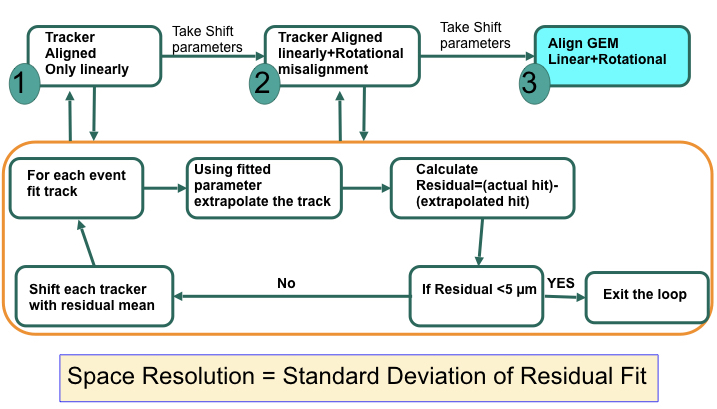
\includegraphics[width=0.95\textwidth]{figures/GEM/GEM_Alignment_FlowChart.jpeg}
    \caption{Alignment algorithm flow chart.}
    \label{fig:alignment}
\end{figure}

\subsubsection{Linear and Rotational Alignment}
To measure the spatial resolution of GEM detectors, these detectors are aligned with respect to the tracker system.
% \subsubsection{Alignment of Reference Trackers}
The first step in the resolution measurement is an alignment of the three small tracking detectors that have a Cartesian X-Y strip readout.
The trackers are first aligned with respect to each other in Cartesian coordinates.
The first alignment step is to shift each of the three tracking detectors iteratively in the XY-plane to make their origins match with each other in that plane.
The initial shift parameters are mean values from position distributions in X and Y coordinates. In each iteration, straight lines are fitted to the hits in X and Y.
In this measurement study, residuals are histogrammed for each detector and the residual distributions are fitted with a double-Gaussian function.
Ten percent of the residual mean value of each detector is taken as the shift parameter in the next iteration to avoid overcorrections.
The resulting residual mean values converge quickly towards zero with iterations and provide a first coarse alignment.
In a second alignment step, we correct also for relative rotations of the tracking detectors around the beam in the XY-plane.
We again fit straight lines to the hits in X and Y and iterate through a succession of offsets and rotations around the beam axis relative to the first tracking detector until the residual means from the trackers are very close to zero and $\chi^2$ of the track fits are minimized.
In each iteration, the detectors are first shifted and then rotated; then new residuals and rotation angles are calculated.
This process is repeated iteratively until the residual means from the track fits becomes less than 0.005 mm. Fig.~\ref{fig:alignment} shows the flow chart of the alignment algorithm.
Figure.~\ref{fig:alignmentIteration} shows the variation of track residuals for three trackers with respect to the iteration number, with residual converging to lower values with each iteration.
\begin{figure}[!htbp]
\centering
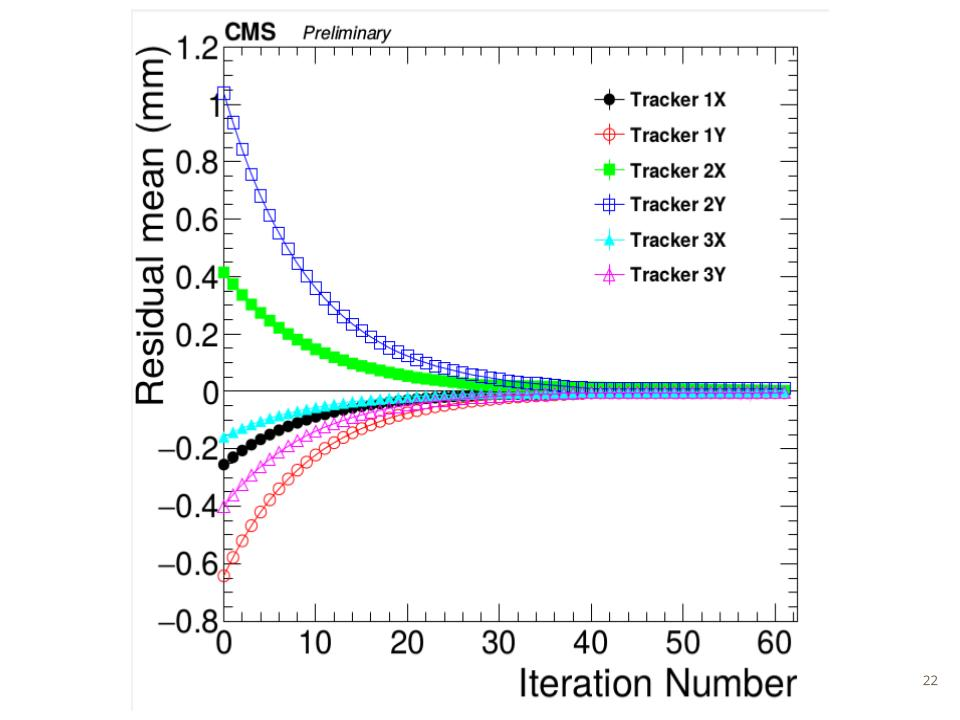
\includegraphics[width=0.65\textwidth]{figures/GEM/Tracker_iterative_alignment.jpg}
\caption{Variation of track residuals for three trackers with respect to the iteration number}\label{fig:alignmentIteration}
\end{figure}

\subsubsection{Alignment GEM detectors w.r.t Reference Tracker}
After the tracker alignment, the next step is to align trapezoidal GEM detectors with respect to the centre of the aligned tracker system.
Twofold iteration loop is used, X offset is kept fixed and iterate over Y offset values with a small fixed step, ranging in a practical phase space. Then X offset is iterated and corresponding iterations are performed with Y offset. For each value of (X offset, Y offset) pair, tracks are linearly fitted in the $\phi$ co-ordinate and the corresponding residuals are noted and used to align the detectors.

\subsubsection{Fiducial Area Selection} % (fold)
\label{ssub:fiducial_area_selection}
To have an efficient efficiency we should define a fiducial area in which we are going to calculate the efficiency. We define the fiducial area as:

\begin{itemize}
        \item For this only \textbf{valid tracks} are considered. Where the valid track is defined as the track that has hit in all three trackers.
        \item Valid tracks are then extrapolated to GE1/1’s and accept that track as a hit in GE11’s if and only if the residual is less than 5 $mm$.
        \item Now two different 2-D histogram is filled. The first histogram contains all those events that have a valid hit in tracker only, as shown in Fig.~\ref{fig:fiducial_area_sel} (left). Another 2-D histogram filled with all those events where there are valid hits in all three trackers as well as the GE11, as shown in Fig.~\ref{fig:fiducial_area_sel}(right).
        \item The ratio of the two histograms defined above is computed, which is shown in Fig.~\ref{fig:fiducial_area_sel} (bottom)
        \item Finally, the region in the ratio histogram where efficiency is maximum is considered as the fiducial region. This fiducial region is considered for the efficiency calculation.
\end{itemize}
\begin{figure}[htbp]
    \centering
    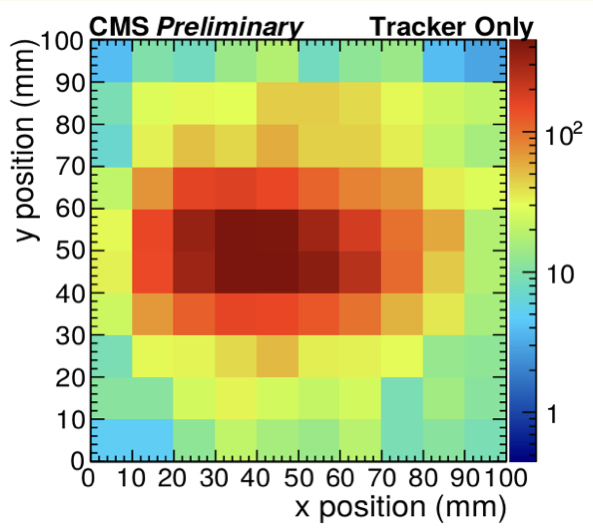
\includegraphics[width=0.45\textwidth]{figures/GEM/FiducialAreaCal_TrackerOnly.jpeg}%
    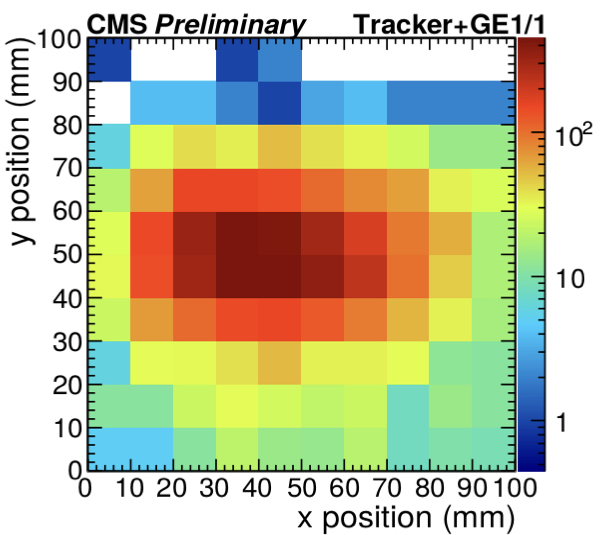
\includegraphics[width=0.45\textwidth]{figures/GEM/FiducialAreaCal_TrackerGE11.jpeg}\\
    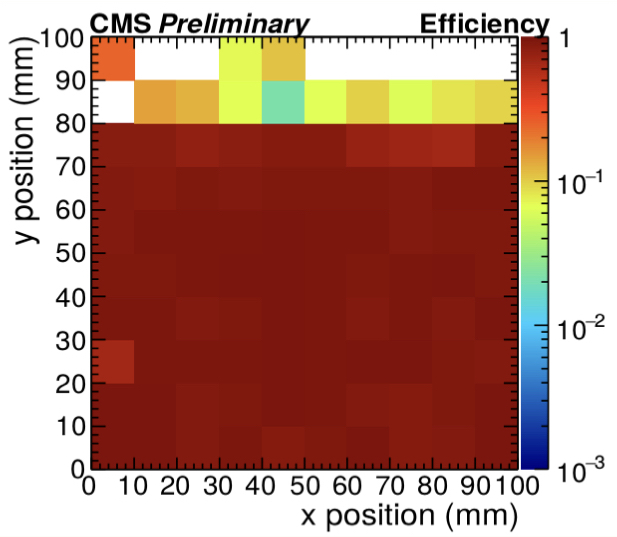
\includegraphics[width=0.55\textwidth]{figures/GEM/FiducialAreaCal_Selection.jpeg}\\
    \caption{Fiducial area selection.}
    \label{fig:fiducial_area_sel}
\end{figure}
% subsubsection fiducial_area_selection (end)
\subsubsection{Efficiency Measurement}
Efficiency, $\epsilon$, is one of the most important parameters for the gaseous detectors. Here it is defined as 
\begin{equation}
\epsilon = \frac{N_{GE1/1+Trk}}{N_{Trk}}
\end{equation}
where $N_{Trk}$ is the number of reconstructed events by using a linear fit $y = mx + b$ fit to the tracker hit positions, in the tracker with normalized $\chi^2<10$.
$N_{GE1/1+Trk}$ is the number of reconstructed events for which an actual hit is found in the GE1/1 within $5mm$ of an extra-plotted track.
The fiducial region in which efficiency was calculated is (0,80) as shown in the previous section.
We are showing here the efficiency as a function of current supplied to high-voltage divider as well as $E_{gain}$, Fig. \ref{Efficiency}. 
\begin{figure}[!htbp]
\centering
% 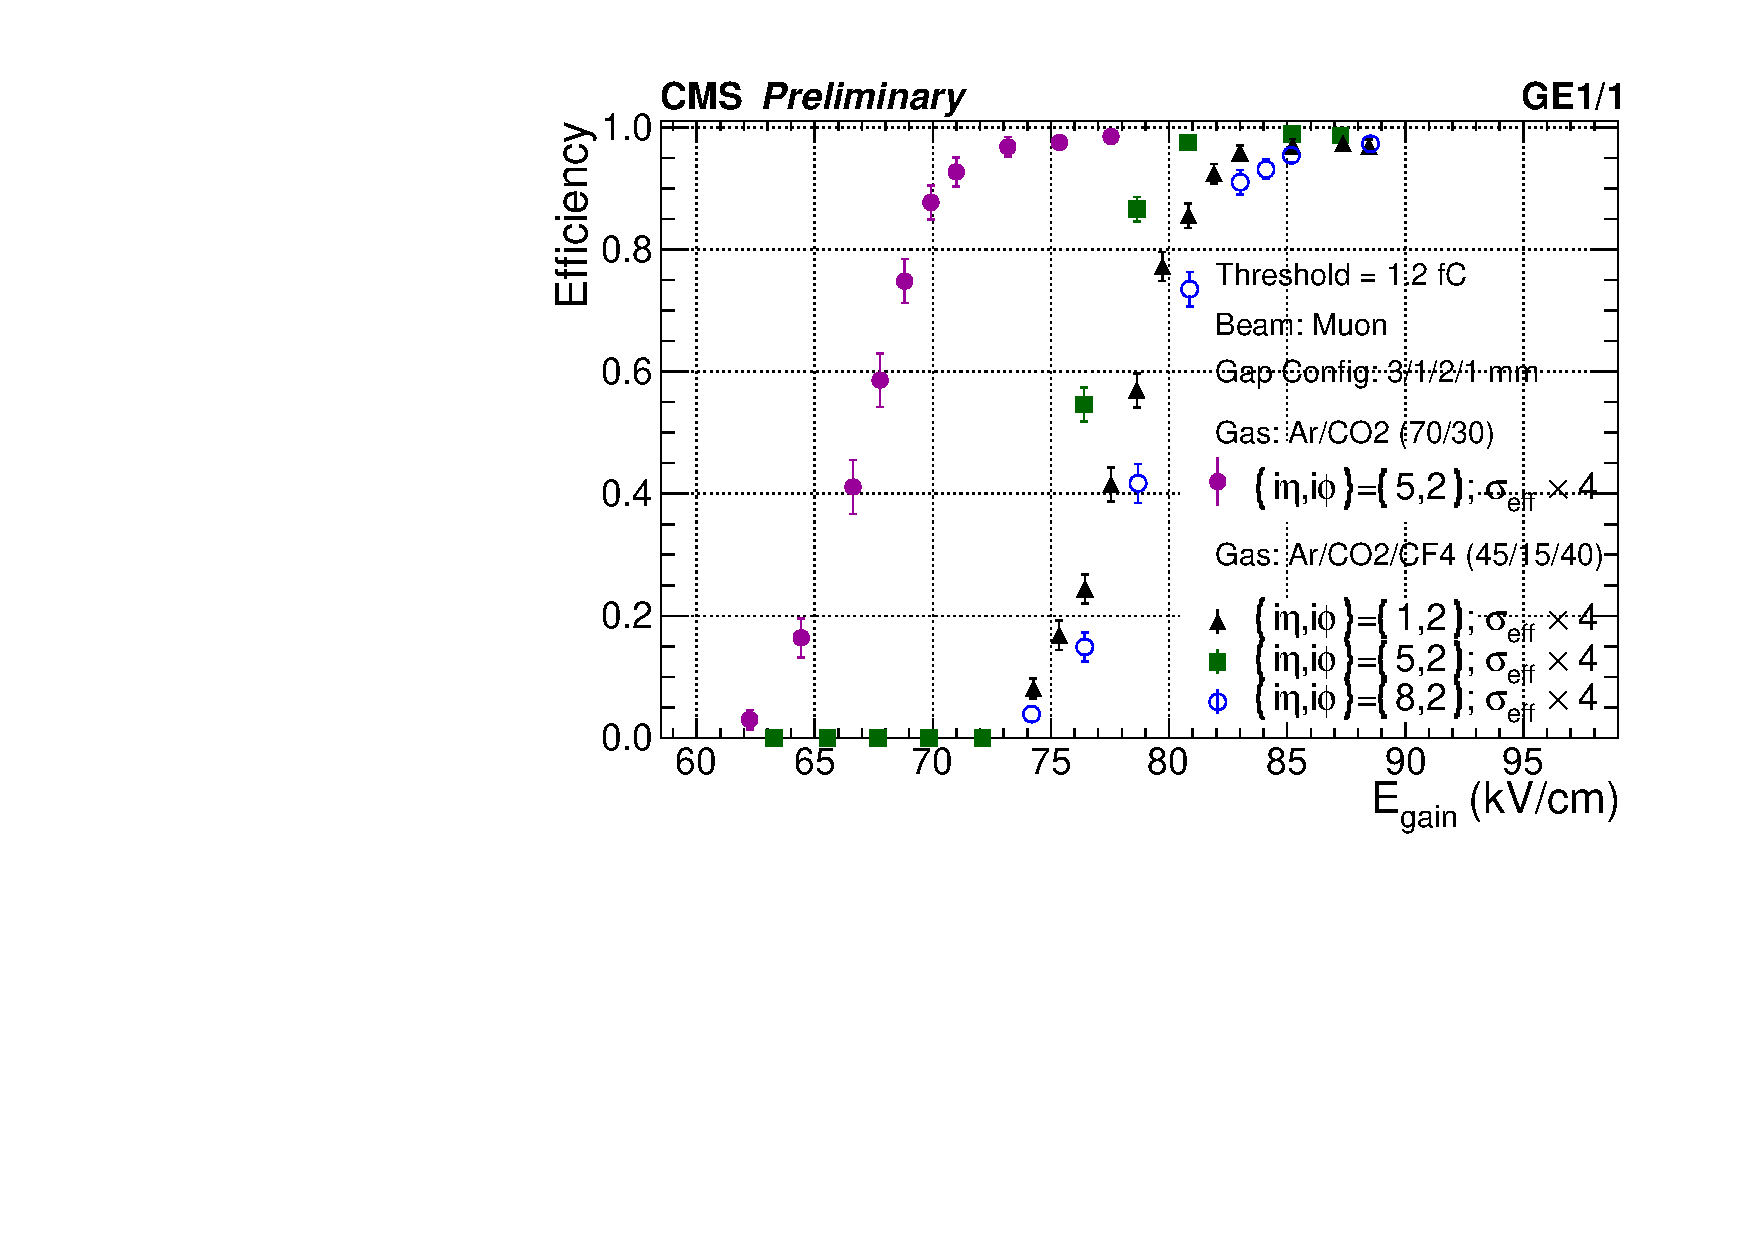
\includegraphics[width=3.5in]{figures/GEM/EfficiencyPlot_wrt_EGain_wError4times_2gas.pdf}
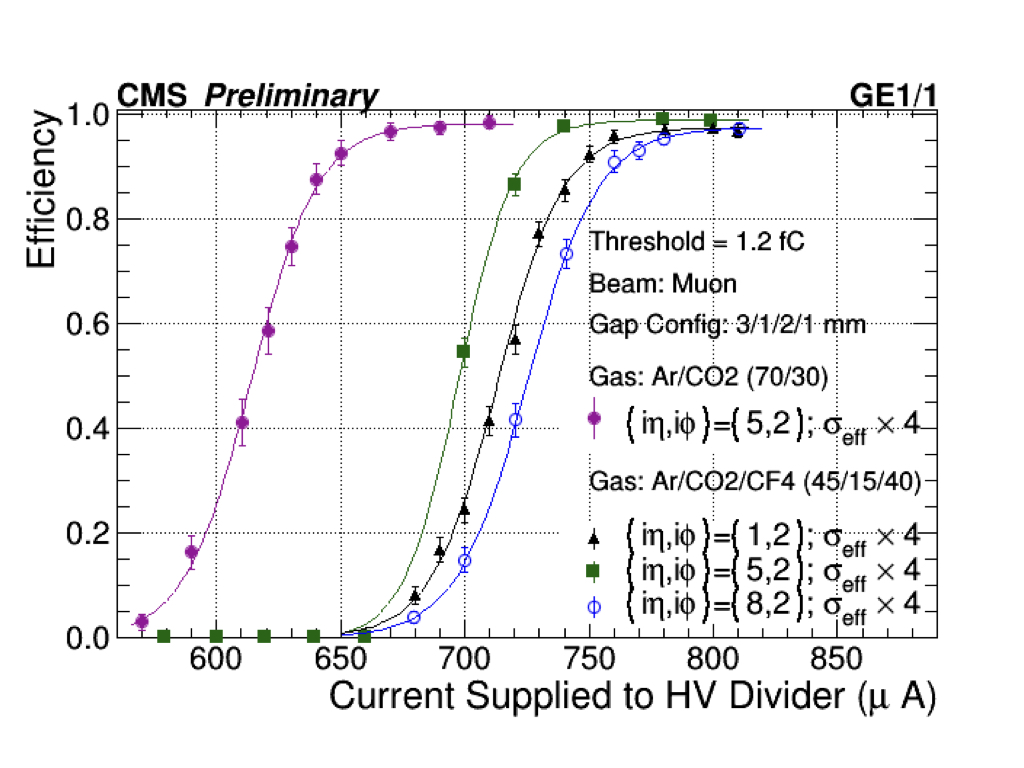
\includegraphics[width=0.75\textwidth]{figures/GEM/Efficiency_Current.jpeg}\\
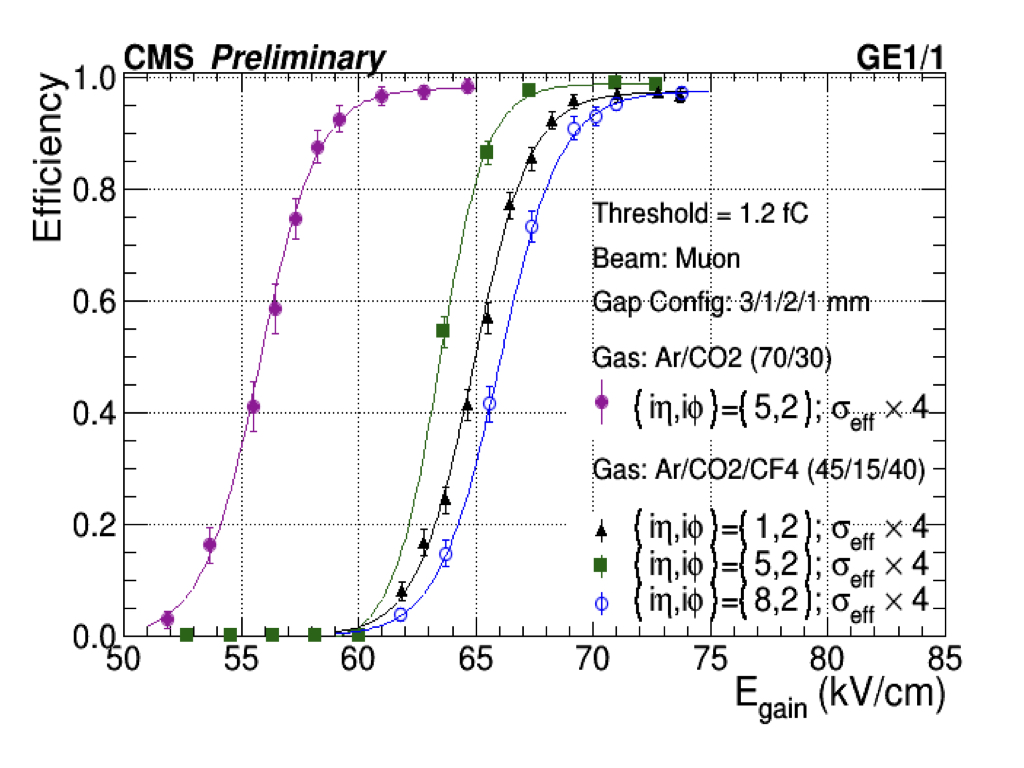
\includegraphics[width=0.75\textwidth]{figures/GEM/Efficiency_EGain.jpeg}
\caption{Efficiency with respect to $E_{gain}$ for two different gases and three different $(i\eta,i\phi)$ sectors.}
\label{Efficiency}
\end{figure}
Where $E_{gain}$ is defined as
\begin{equation}
E_{gain} = \frac{I\times R_{avg}^{gap}}{D}
\end{equation}
Where $I$ is current supplied to the HV divider, $R_{avg}^{gap}$ is the average gap resistance of GE1/1, and D is the thickness of GEM foil.
Here, the efficiency is fitted with function:
\begin{equation}
    Efficiency = \frac{Eff_{max}}{1+e^{s(HV-HV_{50\%})}}
\end{equation}
Where, $Eff_{max}$ is the maximum obtained efficiency, $HV_{50\%}$ is the applied HV (or current or $E_{gain}$) when corresponding efficiency becomes 50\% and $s$ is just a scale factor.

Fig. \ref{Efficiency} is showing the efficiency with respect to two different gas mixtures $Ar/CO_2$ (70/30) at sector $(i\eta,i\phi)=(5,2)$ and $Ar/CO_2/CF_4$ (45/15/40) scanned at three different sectors $(i\eta,i\phi)=\{(1,2),(5,2),(8,2)\}$. We achieved very good efficiency of $\sim$ 98\% in all cases. While for gas mixture $Ar/CO_2$ the threshold is shifted as compared to the $Ar/CO_2/CF_4$ because at fixed high voltage operating point, the effective gain with $Ar/CO_2$  mixture is approximately one order of magnitude higher than $Ar/CO_2/CF_4$ mixture. Also, this shows that we can operate our detector without using the $CF_4$ gas, which is non-environment friendly, without compromising with the efficiency.
      

\subsubsection{Timing Measurement}
The time resolution of a detector is defined as the minimum gate width necessary on the detection electronics for full efficiency.
Experimentally, the time resolution is the root-mean-square of the Gaussian distribution of the time taken by the particle to reach detector from the scintillator.
Along with the fast 40MHz (25ns) clock pulse has been used to cope with the LHC bunch crossing. So, the detector time response is modelled as the Gaussian function, $f(t)$, convoluted with a square wave, $g(t)$, having pulse length $f_{clk}=25ns$ to represent discrete sampling. 
%The functions $f(t)$ is given by:
%\begin{equation}
%f(t) = Ae^{-\frac{1}{2}(\frac{t-t_0}{\sigma})^2}
%\end{equation}
%where A is amplitude of Gaussian function, $t_0$  is the mean value of Gaussian, and $\sigma$ is the standard deviation of Gaussian. And, $g(t)$ is given by
%\begin{equation}
%g(t) =
%       \begin{cases}
%               0, & \text{else} \\
%               1, & \text{$-\frac{f_{clk}}{2}<t<\frac{f_{clk}}{2}$}
%       \end{cases}
%\end{equation}
%where, $f_{clk}$ is the length of created 40MHz window.
The convolution of the two functions is
\begin{equation}
(f*g)(t) = A \cdot \sigma \sqrt{\frac{\pi}{2}}\Big(erf\Big(\frac{u_{+}}{\sigma\sqrt{2}}\Big)-erf\Big(\frac{u_{-}}{\sigma\sqrt{2}}\Big)\Big)
\end{equation}
where $A$ is the amplitude of the Gaussian function, $\sigma$ is the standard deviation of Gaussian, and $u_{\pm}= t-t_0\pm\frac{f_{clk}}{2}$. 
We fitted the experimental data with this convoluted function. From, the fit we extract the time resolution of the detector before the convolution. The time resolution as a function of $E_{drift}$ is shown in Fig. \ref{TimeResolution}. 

Here, the time resolution  with gas $Ar/CO_2$ is fitted with the polynomial of order 2, while with gas $Ar/CO_2/CF_4$ was fitted with the polynomial of order 6.

The time resolution with $Ar/CO_2$ (70/30) is higher for lower values of $E_{drift}$.
However, for any given point on the $Ar/CO_2$ curve has a gain approximately one order of magnitude higher gain than the corresponding gain with $Ar/CO_2/CF_4$ (45/15/40).  We are able to reach faster timing at lower gains with the addition of the $CF_4$ and this is important from the point of view of detector safety because this will allow us to operate the detector at lower gains, hence reducing the discharge probability.

\begin{figure}[!htbp]
\centering
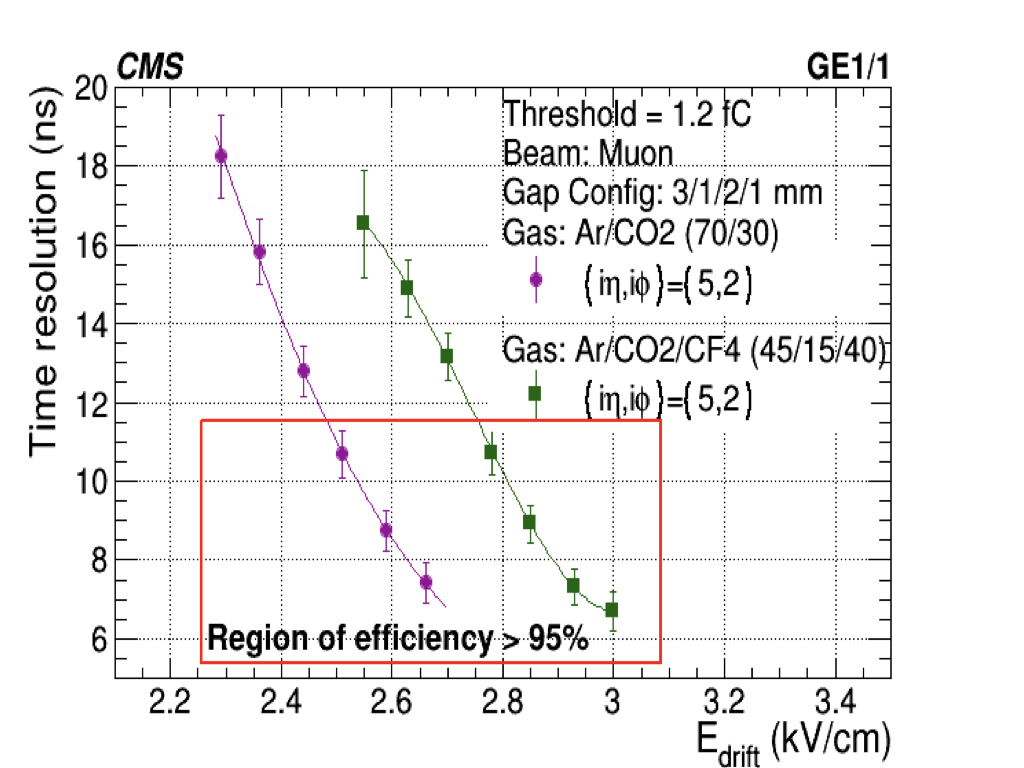
\includegraphics[width=0.75\textwidth]{figures/GEM/TimeResolution_Edrift.jpeg}\\
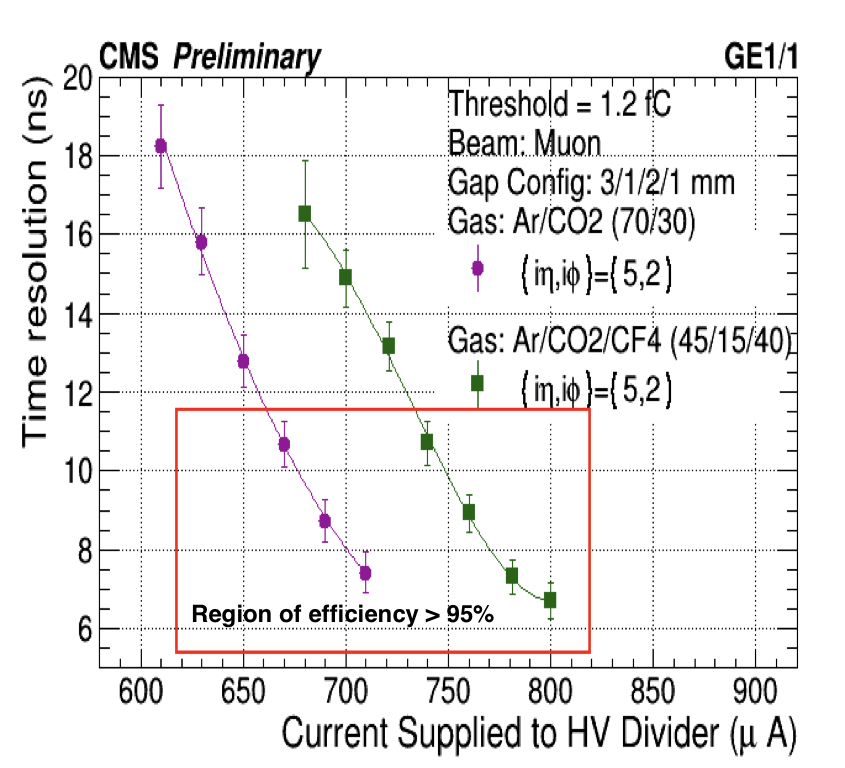
\includegraphics[width=0.75\textwidth]{figures/GEM/TimeResolution_Current.jpeg}\\
\caption{Time-resolution with respect to $E_{drift}$ for two different gases.}
\label{TimeResolution}
\end{figure}



\subsubsection{Cluster Size Study}

Cluster size is defined as the average number of readout strips sharing charge from ionisation of single charged particles.
To study the cluster size, clusterization algorithm is used. The basis of this algorithm is that we considered clusters if there are one or more continuous strips are fired.
Three golden run ranges are studied with different eta sector are 2014H4A, 2014H4C and 2014H4D.
The description of these runs are given in Table~\ref{tab:gemTBgoldenruns}.

To fit the cluster size distribution, Poisson function is used that calculates the number of events in specified intervals. Figure~\ref{fig:CSDpoissonfunction} shows the cluster size distribution for different ($\eta$, $\phi$) sector fitted with the Poisson distribution function.
\begin{figure}[!htbp]
    \centering
    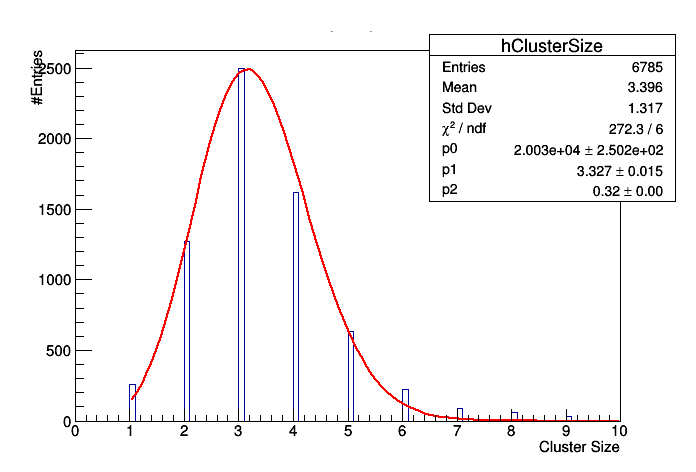
\includegraphics[width=0.45\textwidth]{figures/GEM/Run1644.png}%
    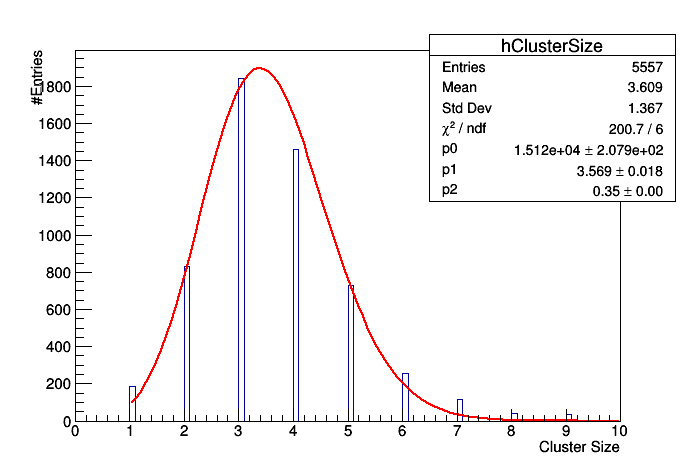
\includegraphics[width=0.45\textwidth]{figures/GEM/Run1869.png}\\
    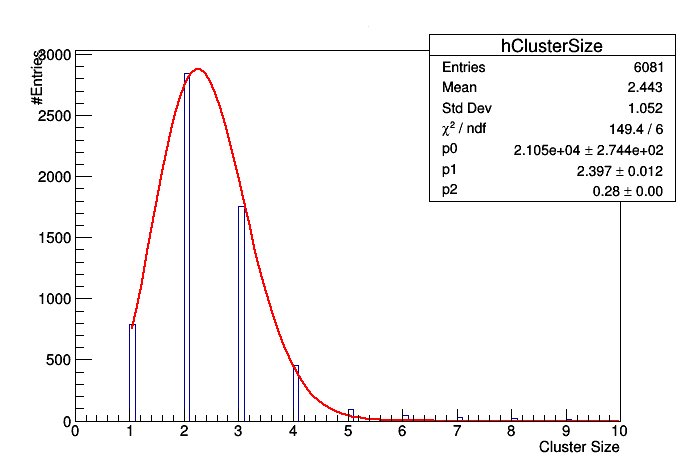
\includegraphics[width=0.45\textwidth]{figures/GEM/Run2066.png}
    \caption{Left: Cluster size distribution for Run1644 in ($\eta$, $\phi$) = (5,2), Right: For Run1869 in ($\eta$, $\phi$) = (8,2), Bottom: For Run2066 in ($\eta$, $\phi$) = (1,2)}
    \label{fig:CSDpoissonfunction}
\end{figure}
Study for the cluster size is done only for the three above mentioned golden run ranges. Distribution is studied with the different fiducial region (full exposed area of the detector). Figure~\ref{fig:CSDfiducialregion} shows that the cluster size is independent of the fiducial region.
\begin{figure}[!htbp]
    \begin{center}
      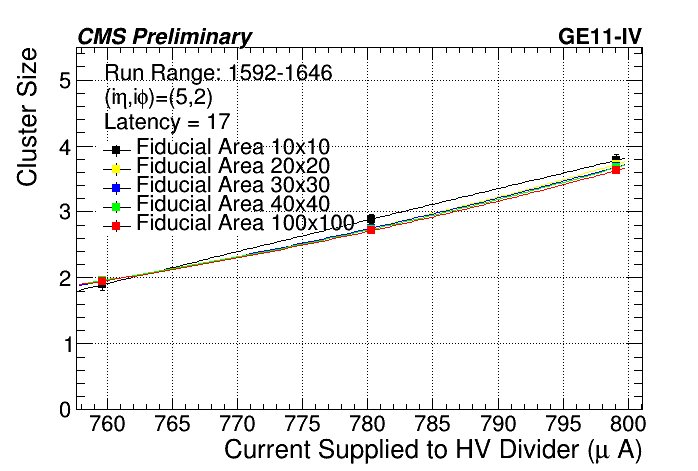
\includegraphics[width=6cm,height=6cm]{figures/GEM/CurrentvsClusterSizeR1592R1646.png}%
      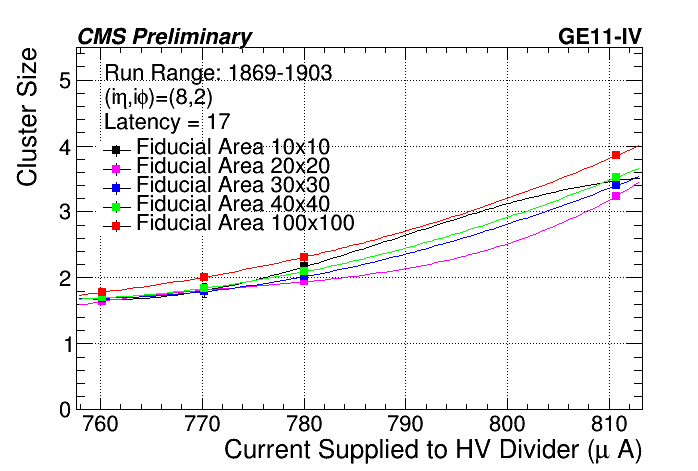
\includegraphics[width=6cm,height=6cm]{figures/GEM/CurrentvsClusterSizeR1869R1903.png}\\
      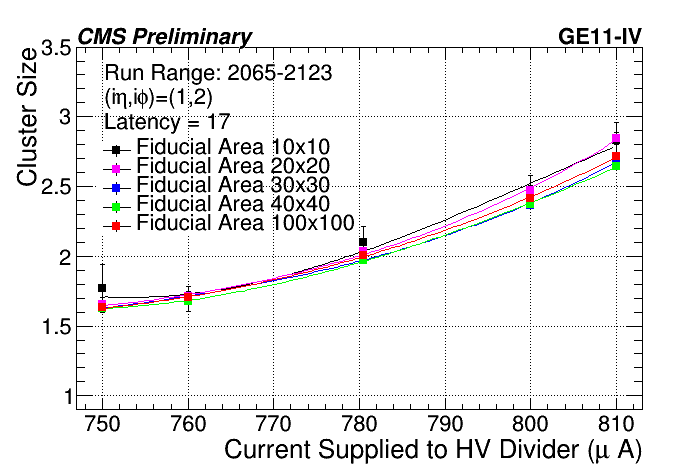
\includegraphics[width=6cm,height=6cm]{figures/GEM/CurrentvsClusterSizeR2065R2123.png}
    \end{center}
    \caption{Cluster size distribution with different fiducial region: Left - Run1592\_R1646 in ($\eta$, $\phi$) = (5,2), Right - Run1869\_R1903 in ($\eta$, $\phi$) = (8,2), Bottom - Run2065\_R2123 in ($\eta$, $\phi$) = (1,2)}
  \label{fig:CSDfiducialregion}
\end{figure}
\begin{figure}[!htbp]
   \begin{center}
     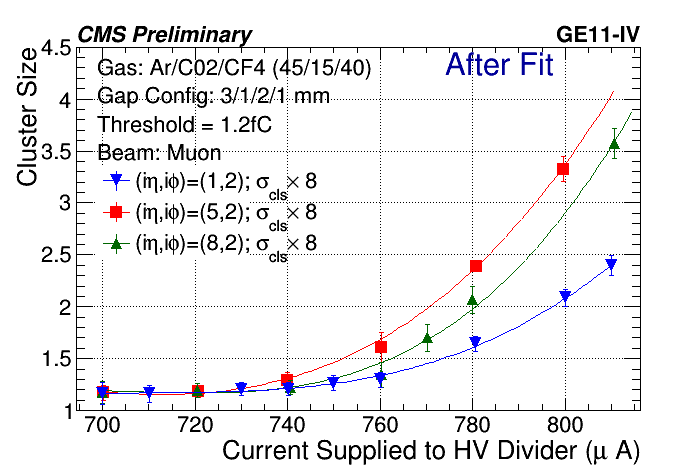
\includegraphics[width=6cm,height=6cm]{figures/GEM/CurrentvsClusterSizeAll3EtaPhi.png}%
     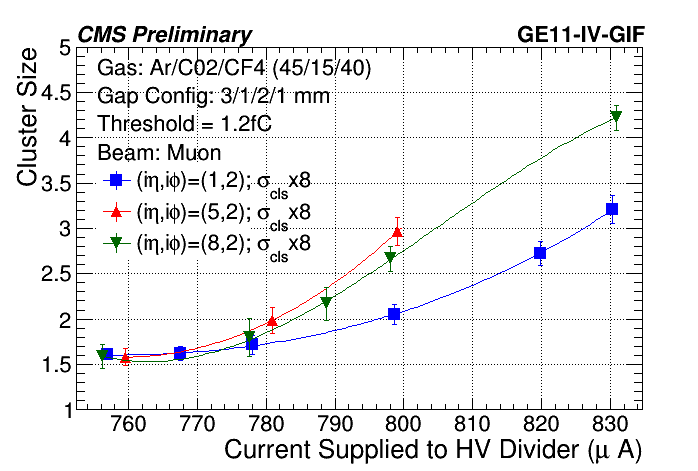
\includegraphics[width=6cm,height=6cm]{figures/GEM/CurrentvsClusterSizeAll3EtaPhiGE11IVGIF.png}
   \end{center}
   \caption{Cluster size distribution: Left - GE1/1-IV, Right - GE1/1-IV-GIF}
   \label{fig:CSDGE1/1}
\end{figure}
Final cluster size study distributions for the GE1/1-IV and GE1/1-IV-GIF\footnote{This is also a generation IV GE11 detector. But, for the ageing test this detector was placed at the Gamma Irradiation Facility (GIF) for twelve months. The GIF bunker contains a $^{137}Cs$ source of 566 GBq. This emits gamma rays of 662 keV. The detector was placed 30 cm from the source where the particle rate was of the order of 100 $kHz/cm^2$. This allowed accumulating the charge in twelve month which will be equivalent to the 10-year operation of GEM detector in LHC environment~\cite{Merlin2013}.} are plotted with respect to the current supplied to the high voltage divider and shown in Figure~\ref{fig:CSDGE1/1}.
Cluster size is taken with the Poisson fitting function. The cluster size is greater in ($\eta$, $\phi$) = (1,2) region for both the detectors due to the uniformity in readouts channels.
% subsection results (end)

% section gem_for_cms (end)

\section{GEM Foil Production and Characterization} % (fold)
\label{sec:gem_foil_production_and_characterization}
Through the Transfer of Technology (TOT) agreement with CERN, Micropack (a Banguluru based Pvt. Ltd. company) signed an agreement for the development of GEM foil in India in collaboration with the Indian Institution.
Micropack started producing the $10~cm~\times~10~cm$ GEM foil using the single mask technique, as this is the one used in GE11 detectors which will be installed in the CMS.
But, after continuous effort and several trials they realized that single mask GEM foil production is the quite challenging method.
Then they switched to the double mask technique and quickly they succeeded with this method. 
They used the similar method used at CERN PCB workshop~\cite{DEOLIVEIRA2009}. 

Micropack used the Kapton foil having a thickness of 50 $\mu m$ with 5 $\mu m$ of copper coating on either side of Kapton foil. Fig.~\ref{fig:Foil_and_Cone_a} shows the $10~cm~\times~10~cm$ GEM foil produced by Micropack and the cross-sectional view of its double conical hole is shown in Fig.~\ref{fig:Foil_and_Cone_b}.
\begin{figure}[!htbp]
    \centering
    \begin{subfigure}[b]{0.46\textwidth}
        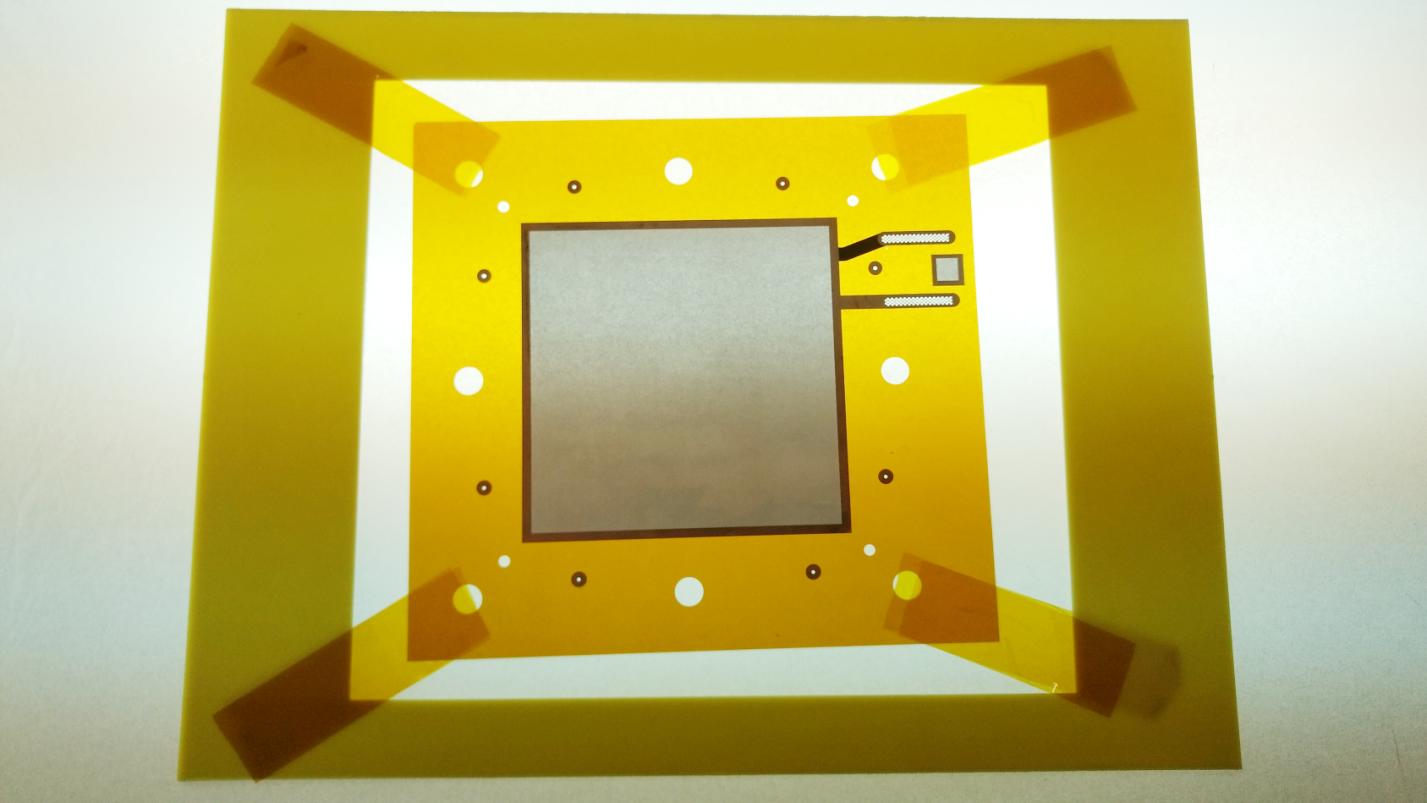
\includegraphics[width=6cm, height=4cm]{figures/GEM/figures/Foil_01.png}\qquad
        \caption{ }
        \label{fig:Foil_and_Cone_a}
    \end{subfigure}
    \begin{subfigure}[b]{0.46\textwidth}
        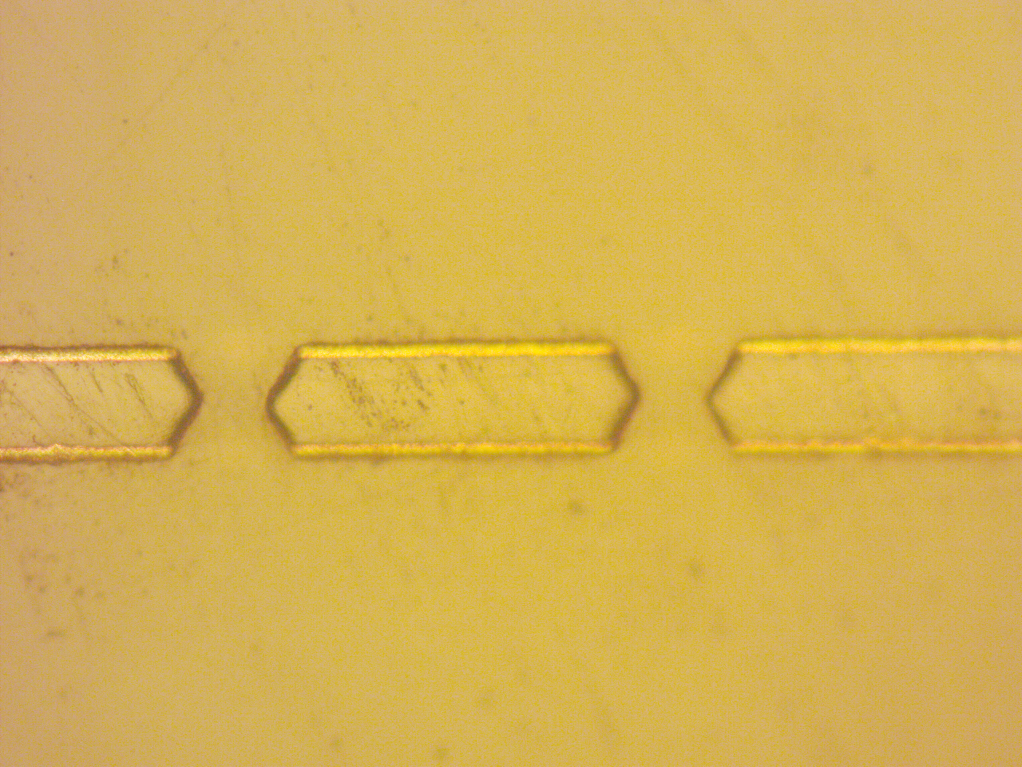
\includegraphics[width=6cm, height=4cm]{figures/GEM/figures/double_cone.png}
        \caption{ }
        \label{fig:Foil_and_Cone_b}
    \end{subfigure}
   \caption{(a) 10 cm $\times$ 10 cm GEM foil encapsulated in a frame and (b) Cross-sectional view of the foil showing the double cone structure of the engraved holes. } \label{fig:Foil_and_Cone}
\end{figure}

To qualify the GEM foil commercially and scientifically reliable it has to pass some quality control test. For a GEM foil the general steps are listed below:
\begin{enumerate}
    \item Visual inspection,
    \item Capacitance and current test of the foil, and
    \item Optical test
\end{enumerate}

Before describing these three inspections one of the important tasks is that one should open/expose the GEM foil only in the clean room\footnote{Clean room is a specially designed room, maintained at extremely low level of particles per cubic meters, for a specialized industrial production or scientific research. For example, a ``\textit{Class-100}'' clean room is designed to never allow more than 100 particles (0.5 microns or larger) per cubic foot of air. ``\textit{Class-1000}'' and ``\textit{Class-10000}'' clean rooms are designed to limit particles to 1000 and 10,000 respectively.} of at least class 100 or less.
As the typical size of GEM holes is 50 $\mu m$ and if it fills up with lots of dust then it will have a destructive discharge as soon as we connect it to the power.
In Delhi University it was done in class 100 clean room installed with KANOMAX dust particle counter model 3887~\cite{KANOMAX-dust-particle-counter} which monitor particle count.
Also, the clean room is equipped with the dehumidifier for humidity control.


\subsection{Visual Inspection} % (fold)
\label{sub:visual_inspection}
At first one has to inspect visually for dust particles and major defects visible to the eye.
If things seem fine then one has to clean it using the adhesive roller, as shown in Fig.~\ref{fig:adhesive_roller}.
\begin{figure}[htbp]
    \centering
    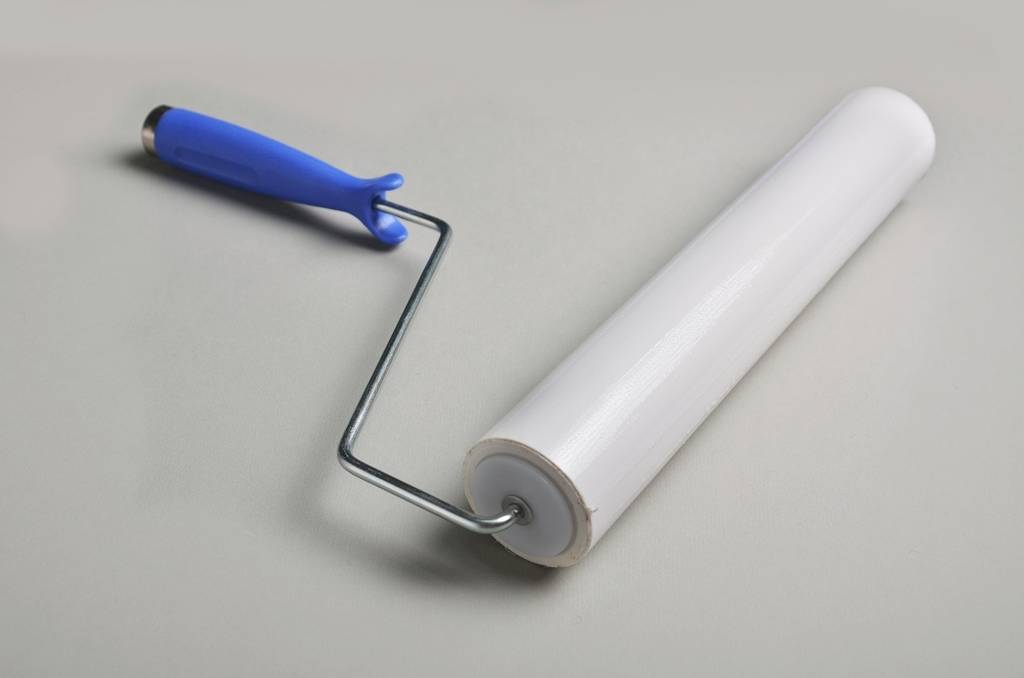
\includegraphics[width=0.55\textwidth]{figures/GEM/Adhesive_roller.jpg}
    \caption{Adhesive roller for cleaning GEM foil.}
    \label{fig:adhesive_roller}
\end{figure}
% subsection visual_inspection (end)

\subsection{Optical Test} % (fold)
\label{sub:optical_test}
Using an optical test we will try to find out:
\begin{itemize}
    \item microscopic defects, which is not visible to the eyes.
    \item Measure the inner and outer hole diameter and pitch size.
\end{itemize}
The motivation for this is the following:
\begin{itemize}
    \item The foil defects such as the over-size hole, missing hole, excess etching, etc will degrade the performance of foil locally.
    \item As the gain depends on the diameter of the hole and the thickness of foil (as shown in Fig.~\ref{fig:gain-vs-holediameter}). So, it will help us to understand the performance of GEM foil such as gain, etc at a later stage.
\end{itemize}
\begin{figure}[htbp]
    \centering
    \includegraphics[width=0.65\textwidth]{figures/GEM/Gain_Vs_Hole_Diameter.png}
    \caption{Real gain and effective gain variation with GEM hole diameter~\cite{Bachmann1999} having a foil thickness of 60 $\mu m$ (= 50 $\mu m$ + 5$ \mu m$ + 5 $\mu m$). As the hole diameter decreases the effective gain increases till 70 $\mu m$ after that it reaches saturation. This is due to loss of generated electrons in the avalanche to the bottom of the GEM electrode when hole diameter is reduced below the foil thickness.}
    \label{fig:gain-vs-holediameter}
\end{figure}
To check the defects and to measure the hole-size and pitch several methods was developed using an automated 2D-CCD scanner~\cite{Posik2015, Becker2006}. 
However, we used a different technique.
We divided the GEM foil into several sectors and captured a high-resolution picture using the AF-S Micro Nikon 40 mm 1:2.8G lens.
We used a softbox ($1~m~\times~1~m$) light source for uniform illuminating the GEM foil.
A sketch of the set-up is shown in Fig.~\ref{fig:Optical_Sketch}.
\begin{figure}[!htbp]
    \centering
    %\begin{subfigure}[b]{0.7\textwidth}
        %\includegraphics[width=12cm, height=8cm]{figures/GEM/figures/NIMA_paper_Images001.jpeg}
        \includegraphics[width=12cm, height=8cm]{figures/GEM/figures/2.jpeg}
        %\includegraphics[width=9cm, height=8cm]{figures/GEM/figures/Optical_Sketch.png}
    %    \caption{ }
    %\end{subfigure}
   \caption{Sketch of the set-up used for the optical measurements.}   \label{fig:Optical_Sketch}
\end{figure}
Fig~\ref{fig:Optical_01} shows the found defects in the considered GEM foil. Also, the measured number of defects is shown in Fig.~\ref{fig:Optical_04}. There is a total of 785 defects found in the GEM foil out of total 600,000 holes in one GEM foil.
Thus there is approximately 0.13\% of defects are there.
Also, a similar number of defects observed in the other two foils. Thus, the local effects in the GEM detector performance should be almost negligible due to the GEM foil defects.
\begin{figure}[!htbp]
    \centering
    \begin{subfigure}[b]{0.29\textwidth}
        \includegraphics[width=4cm, height=3cm]{figures/GEM/figures/3a.jpg}
        \caption{ }
        \label{fig:O_4a}
    \end{subfigure}
    \begin{subfigure}[b]{0.29\textwidth}
        \includegraphics[width=4cm, height=3cm]{figures/GEM/figures/3b.jpg}
        \caption{ }
        \label{fig:O_4b}
    \end{subfigure}
    \centering
    \begin{subfigure}[b]{0.29\textwidth}
        \includegraphics[width=4cm, height=3cm]{figures/GEM/figures/3c.jpg}
        \caption{ }
        \label{fig:O_4c}
    \end{subfigure}
    \centering
    \begin{subfigure}[b]{0.29\textwidth}
        \includegraphics[width=4cm, height=3cm]{figures/GEM/figures/3d.jpg}
        \caption{ }
        \label{fig:O_5a}
    \end{subfigure}
    \centering
    \begin{subfigure}[b]{0.29\textwidth}
        \includegraphics[width=4cm, height=3cm]{figures/GEM/figures/3e.jpg}
        \caption{ }
        \label{fig:O_5b}
    \end{subfigure}
    \centering
    \begin{subfigure}[b]{0.29\textwidth}
        \includegraphics[width=4cm, height=3cm]{figures/GEM/figures/3f.jpg}
        \caption{ }
        \label{fig:O_5c}
    \end{subfigure}
   \caption{Observed imperfections in the foils: (a) Un-etched area, (b) under-size hole, (c) over-size hole (d) missing hole, (e) excess etching and (f) burnt area.} \label{fig:Optical_01}
\end{figure}
\begin{figure}[!htbp]
    \centering
    \begin{subfigure}[b]{0.49\textwidth}
        \includegraphics[width=7.6cm, height=5.5cm]{figures/GEM/figures/Apical_Defects.pdf}\qquad
        \caption{ }
        \label{fig:O_9a}
    \end{subfigure}
    \begin{subfigure}[b]{0.49\textwidth}
        \includegraphics[width=7.6cm, height=5.5cm]{figures/GEM/figures/CopperDefects.pdf}
        \caption{ }
        \label{fig:O_9b}
    \end{subfigure}
   \caption{Number of defects seen in (a) Insulator (Apical Type NP) and (b) Copper, for one of the 10 cm $\times$ 10 cm foil.} \label{fig:Optical_04}
\end{figure}
% subsection optical_test (end)

\subsection{Electrical Test} % (fold)
\label{sub:electrical_test}
This is one of the most important tests which can tell us about the short circuit of the two copper foil, using the leakage current measurement.
Also, it helps us to clean the GEM foil for few dust that can be seen/hear as a spark.
But, if there are the huge number of frequent spark happens then we should quickly stop the electricity and clean the foil properly. In order to qualify the foils the electrical test is divided into two steps as per the CERN standard~\cite{Abbaneo2015}:
\begin{enumerate}
    \item Quality control fast or QC-fast, and
    \item Quality control for long or QC-long.
\end{enumerate}
The difference between QC-fast and QC-long in the two lies in the applying voltage for shorter or longer period of time respectively and monitor the current. Other difference is that QC-fast gives us quick result about the leakage current or electrical connectivity of the foil while QC long provides the behaviour of foil at high voltages and gives us the actual leakage current and the number of discharges if any.
\subsubsection{QC-fast} % (fold)
\label{ssub:qc_fast}
This is done using the insulation tester MIT Megger 420~\cite{twelve}. Using this it is established that the foil has good electrical connectivity. As the 600 V potential is applied across the GEM foil for about a minute and current did not exceed 10 $nA$ and the resistivity in the air between the two foil exceeds 2 $G\Omega$.
% \begin{figure}[!htbp]
%     \centering
%     \includegraphics[width=0.45\textwidth]{figures/GEM/megger.png}
%     \caption{caption}
%     \label{fig:label}
% \end{figure}
% subsubsection qc_fast (end)

\subsubsection{QC-long} % (fold)
\label{ssub:qc_long}
For this, the measurement set-up is shown in Fig.~\ref{fig:Cleaning_Measurement}. It consists of GEM foil enclosed in a Plexiglass enclosure in which nitrogen gas was continuously floated. And the foil is connected with the Keithley 6517B picoammeter~\cite{Keithley-6517B-picoammeter} interfaced with a computer via a GPIB interface and the LabView program was used to record the measurement. The leakage current was measured as a function of applied voltage as shown in Fig.~\ref{fig:Indian_foils_H20}. Also, for the comparison of the same measurement was made with the $10~cm~\times~10~cm$ GEM foil produced at CERN. The results using the CERN foil is shown in Fig.~\ref{fig:CERN_foils}. Thus it is observed that the two foils one produced by Micropack, an Indian Pvt. company and another produced at CERN shows similar behaviour and the leakage current is under the defined limit of 10 $nA$.
% subsubsection qc_long (end)
\begin{figure}[!htbp]
    \centering
    %\begin{subfigure}[b]{0.7\textwidth}
        \includegraphics[width=12cm,height=8cm]{figures/GEM/figures/10.jpeg}
        %\includegraphics[width=12.0cm, height=9.0cm]{figures/GEM/figures/Electrical_Sketch.png}
    %    \caption{ }
        %\label{fig:Setup}
    %\end{subfigure}
   \caption{Sketch of the set-up used for the measurement of leakage current.} \label{fig:Cleaning_Measurement}
\end{figure}
%=====================================================================
\begin{figure}[!htbp]
    \centering
    \begin{subfigure}[b]{0.5\textwidth}
        %\includegraphics[width=7.5cm, height=5.5cm]{Indian_foils_H20.pdf}
        \includegraphics[width=7.5cm, height=5.5cm]{figures/GEM/figures/Fig_11(a).pdf}
        \caption{ }
        \label{fig:Indian_foils_H20}
    \end{subfigure}
    \begin{subfigure}[b]{0.46\textwidth}
        %\includegraphics[width=7.5cm, height=5.5cm]{CERN_foils.pdf} 
        \includegraphics[width=7.5cm, height=5.5cm]{figures/GEM/figures/Fig_11(b).pdf} 
        \caption{ }
        \label{fig:CERN_foils}
    \end{subfigure}
   \caption{Leakage Current of (a) Micropack Foils and (b) CERN Foils, at an average temperature of T=27$^{\circ}$C and relative humidity equal to 20\%.} \label{fig:L_01}
\end{figure}

% subsection electrical_test (end)
% section gem_foil_production_and_characterization (end)

% \section{Summary} % (fold)
% \label{sec:summary}
% First time the GEM foils are produced in India using TOT agreement between CERN and Micropack Pvt. Ltd. Micropack 

% Efficiency and time resolution are important parameters for a gaseous detectors. Efficiency is defined as the ratio of events reconstructed by tracker+GEM to the number of events reconstructed by tracker only. Experimentally, the time resolution is calculated using the root mean square of the Gaussian distribution of the time taken by a particle to reach the detector from the scintillator. Further, we applied a fast 40MHz clock pulse to cope up with the LHC bunch crossing. Thus, the detector's time response should be modelled as the Gaussian function convoluted with a square wave function having frequency 40MHz. To achieve the time resolution we fit the experimental data with the Gaussian function convoluted with the square wave and then using fit parameters we extracted the time resolution before convolution. Finally, we obtained the very good time resolution of ~7ns and efficiency ~98\% with both gas mixture Ar/CO$_2$ (70/30) and Ar/CO$_2$/CF$_4$ (45/15/40), as shown in Fig. \ref{Efficiency} and \ref{TimeResolution}.  At the end, by comparing the results of two different gas mixture  we can  conclude that GEM detectors can be operated without using CF$_4$, while maintaining its performance.


% GEM foils were produced for the first time in India under the TOT agreement between Micropack Pvt. Ltd. and CERN. Micropack started the preparations for the GEM foil production in India. The first few attempts saw many deviations from the required quality. With further improvements in etching technology and several rounds of iterations, Micropack finally produced a batch of foils which appeared fine from visual inspection and preliminary checks. However, before these foils could be declared fit for applications and technology as reliable, we had to perform the desired quality assessment and characterization for these foils. For this purpose, we performed optical and electrical tests to check the reliability and usability of the foils. Optical tests reveal that the holes are quite uniform with inner and outer diameters of 49.9 $\pm$ 1.6 $\mu$m and 70.01 $\pm$ 2.02 $\mu$m respectively. Here, the quoted errors are the Gaussian one sigma uncertainty on diameter distributions. A current of less than 1 nA has been observed in dry nitrogen environment from electrical measurements and were in agreement with CERN foils. The measured optical and electrical properties of Micropack foils were found to reflect the desired parameters and are at par with the double mask foils produced at CERN. With the successful production of 10 cm $\times$ 10 cm double-mask GEM foils, Micropack has already extended their infrastructure to handle single-mask technology so that larger foils can be produced in order to ease the commercialization of large area GEM foils.

% section summary (end)